\chapter{System Design and Implementation}

\section{Overview}

This chapter presents the reference implementation, Contribution C2: a multi-mode diminished-reality
attention-guidance system running on a consumer Meta Quest 3, built in Unity 6 on Meta's Passthrough
Camera Access sample framework \citep{meta2025}. The system realises the design space of Chapter 3 in
a deliberately economical architecture, \textbf{one shader and one manager component on a single
piece of geometry}, and the economy is itself a result: every capability tier of Chapter 3's taxonomy
is reachable from one head-centred sphere and one fragment program.

Throughout, parameter names in \verb|code font| are the actual serialized fields and shader
properties in the repository (\verb|CameraSphereVignette.shader|,
\verb|CameraSphereVignetteManager.cs|, \verb|VideoTestSceneManager.cs|), so every quantitative claim
is checkable against the artifact. The full repository is publicly available at
\url{https://github.com/batunii/Arjuna}, including the shader and manager sources, the study
harness, the analysis scripts that regenerate every statistic in Chapter 5, and the raw capture
records behind Section 4.11.

\begin{figure}[htbp]
\centering
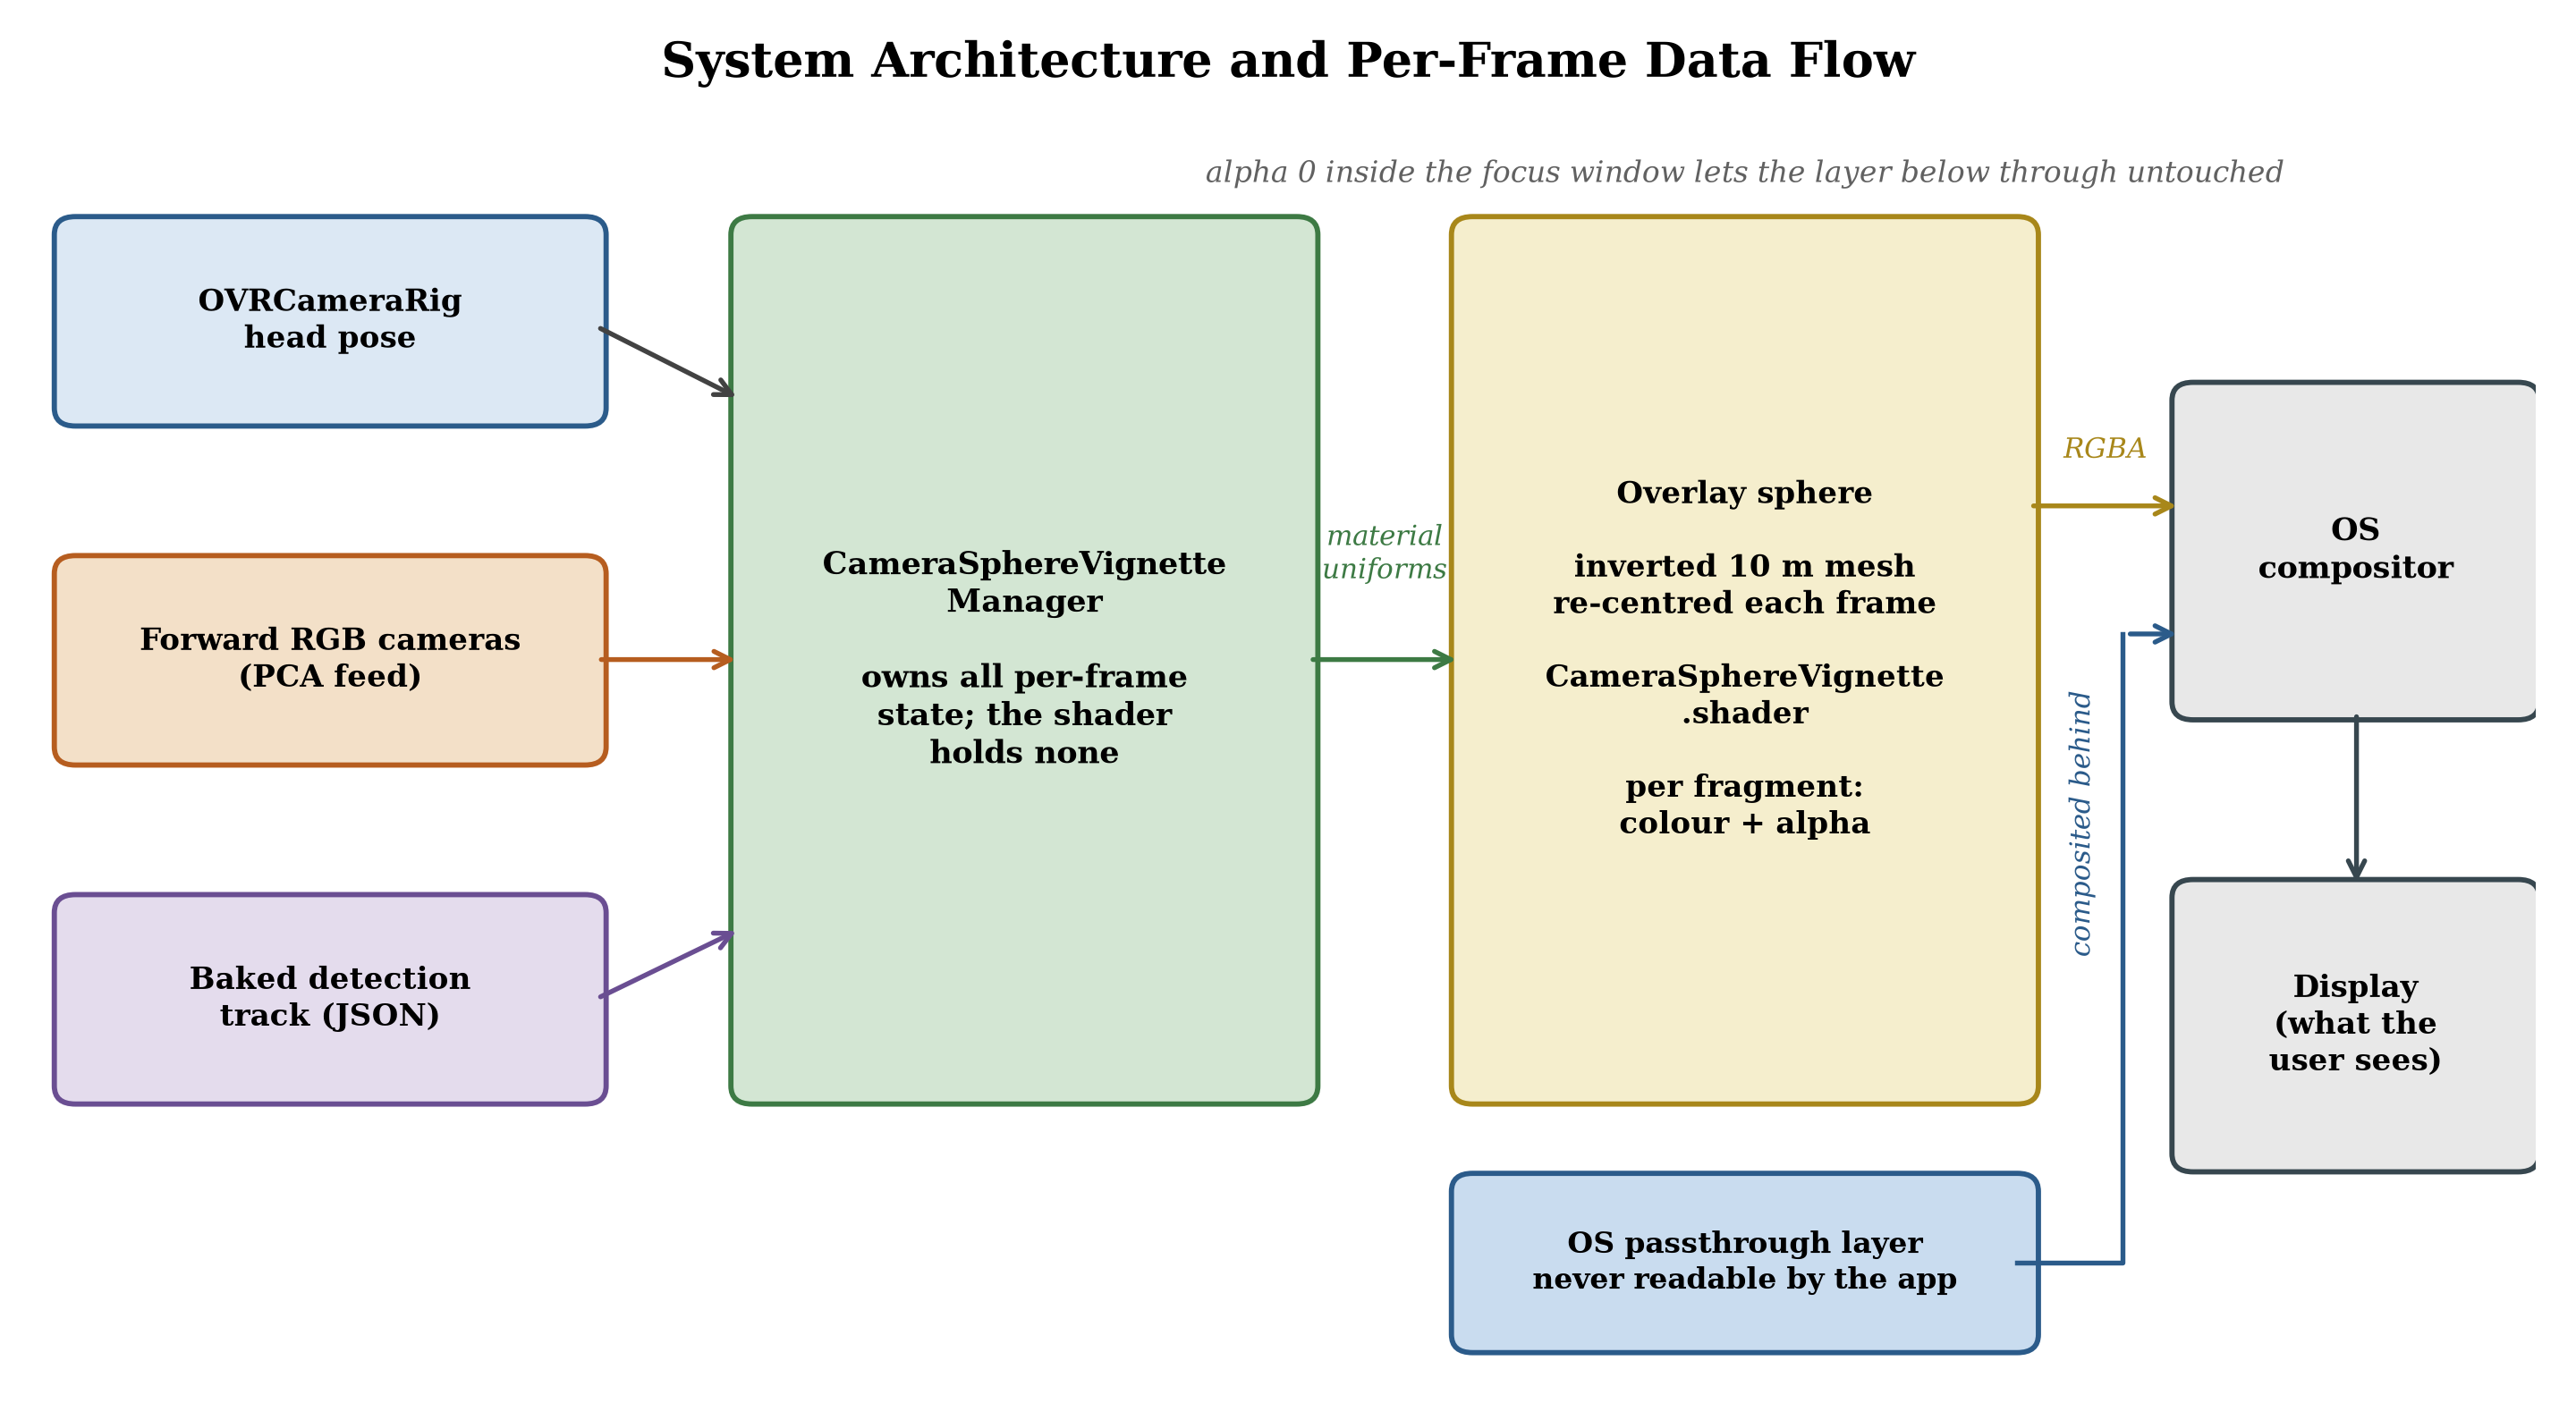
\includegraphics[width=\linewidth]{content/figures/fig_architecture.png}
\caption{System architecture and per-frame data flow.}
\label{fig:architecture}
\end{figure}

Figure~\ref{fig:architecture} shows the components and the per-frame flow between them.

\section{The Sphere and the Window}

\subsection{Geometry}

The entire visual effect is carried by a single inverted sphere of approximately 10 m radius, centred
on the user's head and re-centred every frame. The translation is applied without rotation, which is
what keeps the sphere's surface coordinates world-stable. The mesh is rendered inside-out with
\verb|Cull Front|, on the transparent queue, with depth writes disabled and conventional alpha
blending. Every fragment the user can see, in any direction, is a fragment of this sphere. The
shader's output alpha at that fragment decides, per pixel, whether the user sees the diminishment
effect or whatever lies behind the sphere, which in the passthrough scene is the operating system's
native passthrough layer.

This choice of a fragment-alpha-controlled full-surround surface is what makes one object span all of
Chapter 3's tiers. Alpha 0 is Tier 2's absence, so native passthrough passes through untouched. Alpha
1 with a black colour is Tier 2's blackout. Alpha 1 with a camera-fed colour is Tier 3's re-render.
The mode logic reduces to deciding, per fragment, a colour and an alpha.

\subsection{The world-locked focus window}

Two different things in this system can look similar, and the chapter keeps them apart by name. The
\textbf{focus window} is the region the user places and locks onto a spot in the room. It stays fixed
to that spot, the application draws nothing inside it, and it does not move again until the user
resets it. The \textbf{detection aperture} is a smaller opening the system creates over an object a
detector has just recognised. It appears and disappears as objects are recognised and lost, and the
user has no control over it. Section 4.5.5 describes the aperture.

The focus window is stored not in screen space or head space but in \textbf{world spherical
coordinates}: a rectangle \verb|_FocusRect = (azMin, azMax, elMin, elMax)| in radians of azimuth and
elevation about the sphere's centre. Each fragment reconstructs its own direction from first
principles:

\begin{verbatim}
dir = normalize(worldPos - _SphereCenter)
az  = atan2(dir.x, dir.z)
el  = asin(dir.y)
\end{verbatim}

and computes a signed distance outside the rectangle, \verb|max(dAz, dEl)|, which a smoothstep
across the soft edge converts into the per-fragment vignette coordinate \textbf{t}: 0 inside the
window, rising smoothly through the soft edge, and 1 in the far periphery. Every mode
consumes this single scalar. The dark modes use it directly as overlay alpha. ColorPop uses it to
interpolate each pixel between its inside and outside treatments.

The soft edge defaults to \verb|m_softEdgeDeg| = 20$^{\circ}$, widened to 32$^{\circ}$ for ColorPop
(Section 4.5.2). These are the component defaults. The two evaluated modes serialise different
values, for reasons that follow from what each is for. SignPop, as a colour-pop mode, takes the
widened edge at 24$^{\circ}$, because a colour-to-grey boundary reads harsher than a dark one.
Hard Dark takes a deliberately narrow 2$^{\circ}$ edge (\verb|m_hardDarkSoftEdgeDeg|), because its
role is the strongest available occlusion: once a selection is locked, everything outside it should
read as black almost immediately rather than fade through a wide gradient buffer. Both run against a
$\pm$8$^{\circ}\times\pm$6$^{\circ}$ window, which is the geometry Chapter 5, Section 5.7.3 reads its
eccentricity bands against. The 20$^{\circ}$ default is chosen against the useful field of view, the region
within roughly 30$^{\circ}$ of fixation from which people extract task-relevant information without
moving their eyes or head \citep{ball1993}. Placing the soft edge inside that radius means the
transition band falls where the eye is still resolving detail, so the effect reaches full strength
just as the useful field runs out rather than cutting sharply across it. It also sits above the
$\approx$15$^{\circ}$ eccentricity beyond which head yaw becomes a reliable pointer to attention
\citep{higgins2022}, which matters because the window is placed by head-directed painting and must be
larger than the noise floor of the pointing method that places it.

Because azimuth and elevation are computed from world direction, the window is \textbf{world-locked}.
It stays fixed to the room, to the desk, the doorway, the whiteboard, as the head rotates, rather
than travelling with the gaze. Direction is computed per-fragment from \verb|worldPos| rather than
interpolated from vertices, which avoids interpolation error at the sphere's poles.
Figure~\ref{fig:window} shows the rectangle on the sphere, the soft-edge band, and the resulting
profile of \textbf{t} along one axis.

\begin{figure}[htbp]
\centering
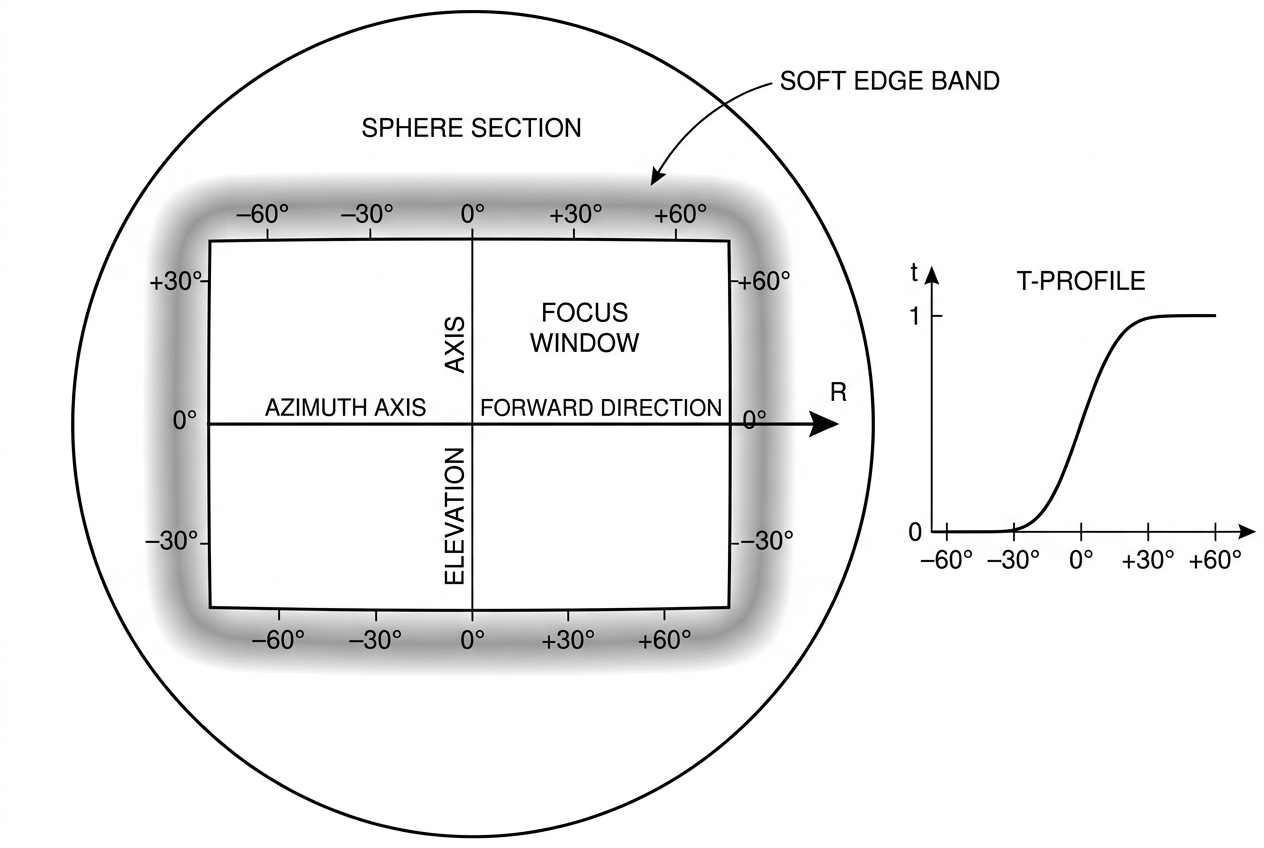
\includegraphics[width=\linewidth]{content/figures/fig_window_geometry.jpg}
\caption{The az/el window geometry.}
\label{fig:window}
\end{figure}

\subsection{The window as absence}

In the passthrough scene the shader's output inside the window is \verb|alpha = t = 0|, so nothing is
drawn. The consequence is the system's central design decision. Inside the window the user sees the
operating system's own passthrough at full native quality, full $\sim$110$^{\circ}$ field of view,
and the OS pipeline's own latency compensation, none of which any application-rendered reconstruction
can match. The effect budget is spent entirely in the periphery, where human acuity is lowest. One
line of shader arithmetic simultaneously solves the field-of-view problem, since the accessible
camera feed covers only $\sim$85–90$^{\circ}$, and the fidelity problem, since that feed is
1280$\times$960 per camera against a native reprojected stereo view, by ensuring the reconstruction is only ever shown
where neither limitation matters much.

\subsection{Per-frame data flow}

The manager owns all per-frame state and feeds the shader exclusively through material uniforms, so
the shader holds no state of its own. Each frame it re-centres the sphere on the head anchor and
uploads \verb|_SphereCenter|, the one value the whole angular coordinate system depends on, the focus
rectangle and soft edge, the combined formation and motion-suppression strength, and the active
mode's parameter block. For camera-fed modes it also uploads each camera's pose basis and half-FOV
tangents, derived from the intrinsics the PCA API reports rather than an assumed field of view, which
is what keeps the camera periphery in scale with the native window across the seam. The shader is
written for single-pass instanced stereo and, by the world-direction design of Section 4.4, contains
\textit{no} eye-dependent sampling anywhere in the camera path, so the renderer needs no per-eye
scripting.

\section{The Hybrid Composite}

The system's flagship configuration composes the tiers: a \textbf{Tier-3 processed camera feed as the
periphery, with the Tier-2 transparent window revealing native passthrough as the focus region}.
These are two different renderings of the same reality, fused into one continuous view.

Mechanically, the PCA feed is bound to the sphere material (\verb|_MainTexL|, and \verb|_MainTexR|
where the right camera is available), the fragment shader computes each periphery fragment's colour
from the feed with whatever manipulation the active mode specifies, and outputs it at
\verb|alpha = t*strength|. Inside the window, \verb|t = 0| yields transparency and the OS layer shows
through. The seam between the two renderings is the window's soft edge, where the processed feed
fades out over \verb|_SoftEdge| radians. Because both renderings depict the same world from nearly
the same viewpoint, the transition tends to read as an effect boundary rather than as two images.

The construction has one honest seam-level caveat. The two renderings do not share a latency budget:
the OS passthrough inside the window is served by the platform's dedicated low-latency reprojection
path, while the camera-fed periphery carries the application pipeline's additional delay. In static
or slowly moving views the mismatch is not noticeable. Under fast head rotation the periphery can
momentarily lag the window at the seam. The motion-based suppression of Section 4.6 incidentally
masks the worst case, since the effect fades out precisely when the head moves fast, but the residual
mismatch is a real property of the hybrid rather than something designed away.

The claim this construction supports is deliberately precise (Chapter 3, Section 3.5): the
\textit{composite} is the novelty, exploiting the quality and field-of-view asymmetry between a
native layer that cannot be touched and a camera copy that can, not any of its ingredients. Its costs
are Tier 3's costs, paid only in the periphery. Figure~\ref{fig:hybridphoto} shows the composite as
recorded on device.

\begin{figure}[htbp]
\centering
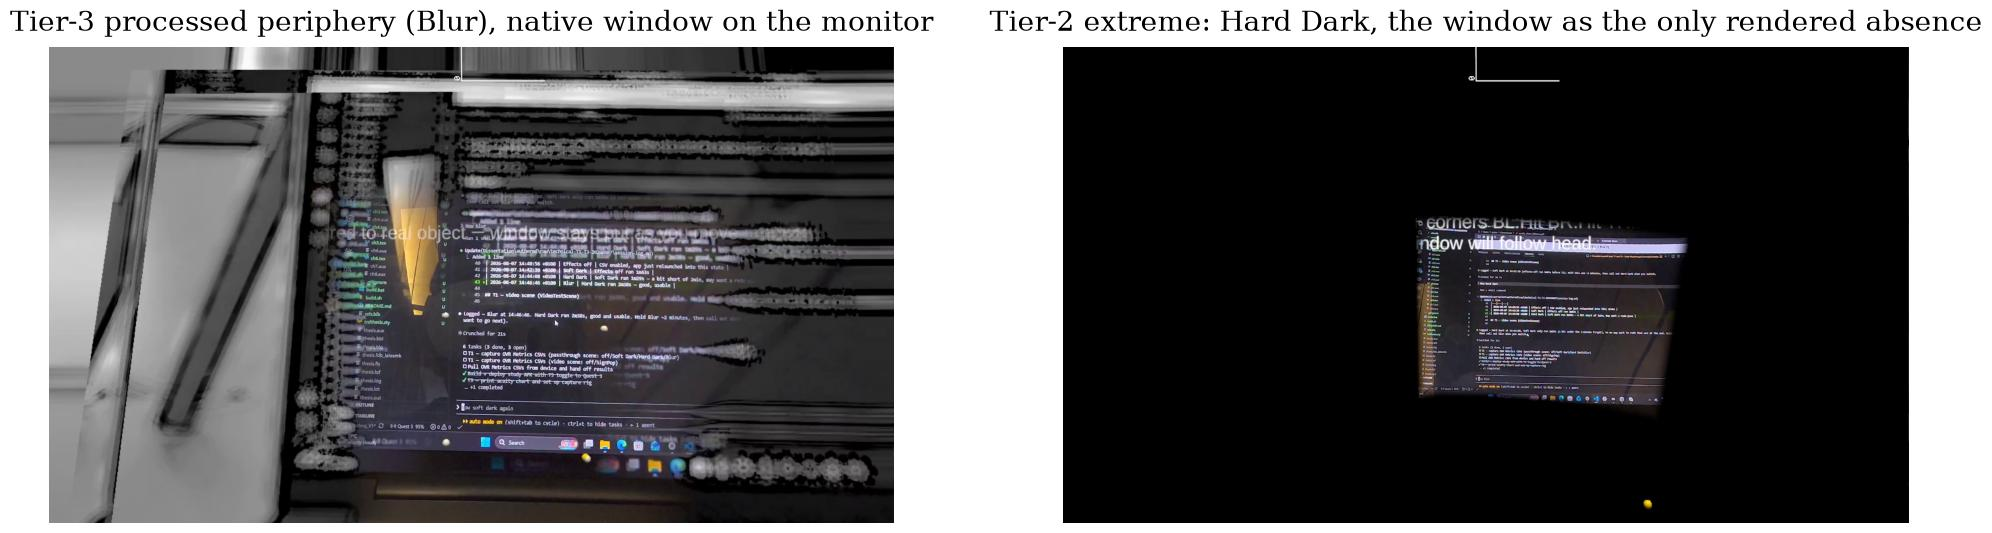
\includegraphics[width=\linewidth]{content/figures/fig_hybrid_photo.jpg}
\caption{The window as absence, from on-device recordings of the same room. Left: a Tier-3 processed
camera periphery (the Blur variant, whose contrast restoration reads as an edge drawing) surrounds
the world-locked window, through which the monitor is served by native OS passthrough in full
colour. Right: the Tier-2 extreme, Hard Dark, where the window is the only region not rendered.}
\label{fig:hybridphoto}
\end{figure}

\section{Binocular Fusion by World-Direction Sampling}

Passthrough Camera Access exposes both forward cameras, but most modes here sample only one, and
every mode must present a camera image that is not eye-aligned to a binocular display. How that
image is presented to two eyes determines whether the system is usable at all. The governing requirement is
that the sampling domain be \textbf{eye-independent}. Under stereo rendering the same world point
projects to different screen positions in each eye, so any scheme keyed to screen position feeds each
eye a different camera pixel for the same world point, and the two images do not fuse
(Section 4.10, failure 1).

The shader therefore samples by \textbf{world direction}. Each fragment's direction from the sphere
centre, already computed for the window test, is projected through a head-centred pinhole model of
the camera. With the camera's forward, right and up basis and half-FOV tangents derived from the
camera intrinsics rather than an assumed field of view, the shader computes

\begin{verbatim}
uv = ( (dir.rt, dir.up) / max(dir.fwd, eps) ) / tanHalfFov * 0.5 + 0.5
\end{verbatim}

Because world direction is eye-independent, both eyes sample the \textit{same} camera pixel for the
same world point. The camera image behaves like a texture painted onto the world shell, which the
visual system can fuse, as verified on device (Section 4.10). The residual and acceptable artefact is that the painted shell has no true stereo
disparity of its own, which is consistent with the project's standing comfort constraint that a
single-camera feed must never be presented as if it were geometry-correct stereo across the full field of view.

Where both cameras are available, the shader samples both and selects per fragment by in-view weight,
a \textbf{hard split} rather than an alpha crossfade, because a crossfade of two horizontally offset
viewpoints produces exactly the ghosting the world-direction scheme exists to avoid. The two forward
cameras share an orientation and differ only by a small horizontal baseline, and no stitch line was
visible in normal use. Figure~\ref{fig:fusion} contrasts the two sampling schemes on the same world
point.

\begin{figure}[htbp]
\centering
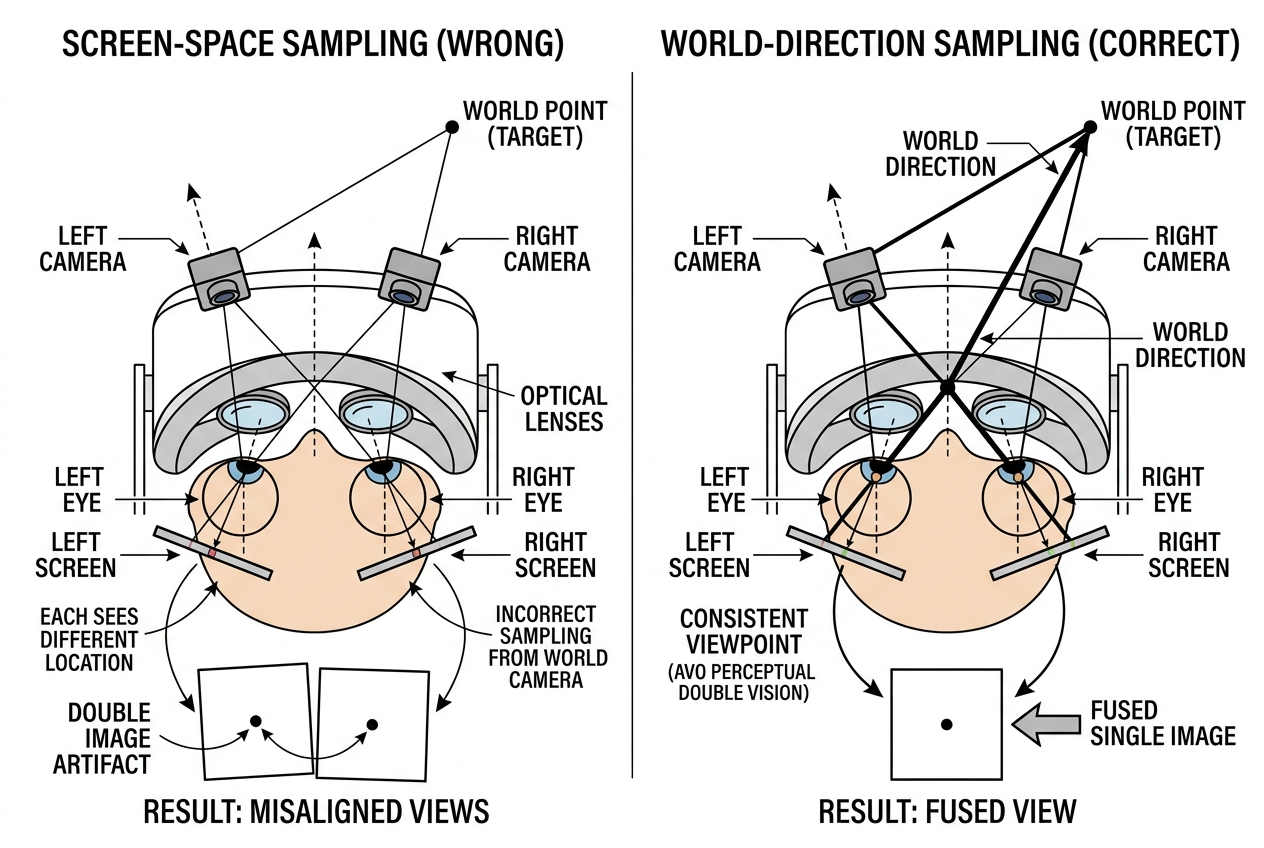
\includegraphics[width=\linewidth]{content/figures/fig_fusion_sampling.jpg}
\caption{Screen-space versus world-direction sampling of a mono camera feed.}
\label{fig:fusion}
\end{figure}

\section{The Modes}

The mode enumeration in the codebase (\verb|VignetteMode|) contains eleven entries. Two are carried
into the user study, SignPop and Hard Dark, both to confirmatory testing. A third, Soft Dark, is
specified here but was never tested with participants (Chapter 3, Section 3.4). ColorPop is the base
grading pipeline SignPop extends with a detection gate. Blur is their superseded ancestor, and five
further entries are retained design-exploration variants. All share the geometry, window, and
t-coordinate of Section 4.2. A mode is, in implementation terms, a per-fragment colour and alpha
policy. Mode names are the code identifiers, kept so every claim stays checkable against the
repository, and where a name suggests a standard image-processing operation the description given
with it is authoritative: Blur, for instance, names a progressive two-ring Gaussian of the camera
periphery with contrast restoration, not a whole-image convolution.

\subsection{Peripheral occlusion (Hard Dark and Soft Dark)}

The simplest and strongest manipulation is a black overlay whose alpha is the vignette coordinate
scaled by the current strength:

\begin{verbatim}
periColor = black
periAlpha = t * _VignetteStrength * _MaxVignetteAlpha
\end{verbatim}

\noindent with \verb|_MaxVignetteAlpha| = 1.0. At full formation the periphery is completely
occluded and the user's visual world \textit{is} the focus window. The shader path (\verb|_SimpleMode = 1|) samples no textures and does no camera mathematics.
An early return delivers what is effectively a fixed-function overlay, with correspondingly
negligible GPU cost and no camera permission or thermal exposure, which is Chapter 3's deployability
argument in code. Hard Dark is the confirmatory mode of the workstation block: the strongest
available manipulation, chosen to maximise the chance of detecting the distraction-suppression
mechanism if it exists.

The same shader path run with \verb|_MaxVignetteAlpha| set from \verb|m_mode2MaxAlpha| (default
\textbf{0.75}) gives Soft Dark, where the periphery darkens substantially but never fully, so
peripheral motion and events stay visible through the veil. The ceiling is set below 1.0 rather than
at it because \citet{cheng2022} found users asked what they want from diminishment prefer partial
opacity reduction to complete removal, and want enough residual structure to know something is still
there. Soft Dark is that preference implemented as a number.

Both dark modes \textbf{form gradually}. On window lock, a coroutine animates
\verb|_VignetteStrength| from 0 to 1 along a SmoothStep over \verb|m_vignetteFormTime| (default
\textbf{3 s}), so the periphery dims as a transition rather than a cut. The ramp is there because
\citet{hata2016} showed a visual change introduced gradually enough stays below the awareness
threshold while still biasing gaze, so the guidance survives the ramp even though the announcement
does not. Formation runs independently of the motion suppression of Section 4.6: if the head moves
during formation, suppression multiplies the strength down while the formation clock keeps counting,
and the effect resumes at its accumulated level when the head settles.

\subsection{Colour- and saliency-gated peripheral re-grading (ColorPop)}

ColorPop is the Tier-3 mode. It re-grades the camera feed's colour and brightness rather than dimming
it, using the literature's strongest guidance channel, luminance and saturation contrast, with no hue
shifts \citep{bailey2009,grogorick2017,sutton2022}. The re-grading is a standing property of the
whole visual field rather than a transient cue that appears and disappears.

Its grading is a \textbf{four-level hierarchy} on two tracks, gated by colour class and interpolated
by the window coordinate t:

\begin{center}
outside-other $<$ outside-ROG $<$ inside-other $<$ inside-ROG
\end{center}

\textbf{Colour classification.} A shader helper computes membership in the kept red, orange and green
(ROG) set, the colour classes of signal lamps and signage. Membership is defined by hue bands, a warm
band and a wrap-around red band above 0.85, plus a green band from 0.22 to 0.48, each gated by a
saturation floor. The warm band uses a deliberately higher floor (\verb|_PopWarmSatMin| = 0.35)
because warm-\textit{white} light, headlights at hue $\approx$ 0.1 and saturation 0.1 to 0.25, must
not ride into the orange class, while genuine lamps and signs sit above saturation 0.5. The floor is
therefore placed in the gap the two populations leave.

\textbf{The other track}, meaning non-ROG pixels, stays near-natural inside the window, with a slight
desaturation that keeps the window from feeling artificially vivid against its own periphery, and is
graded down to dim grey outside (\verb|_PopGreyDim| = \textbf{0.4}). The floor sits at 0.4 rather
than lower because a periphery approaching black would carry almost no peripheral events, and a
monitoring mode whose own dimming floors peripheral detection would fail its safety hypothesis by
construction rather than by finding. This track covers the great majority of peripheral pixels, so
its floor, rather than the signal track's, is what decides whether the periphery stays usable.

\textbf{The ROG track} leaves signal-relevant colour untouched inside the window and attenuates it
gently outside. Inside, saturation and brightness are held at unity, so a kept pixel is passed
through at its natural appearance. Outside, ROG pixels retain their hue but are taken to 55\% of
their chroma and 60\% of their luminance. This is deliberate: signal-relevant colours remain
detectable \textit{everywhere}, merely privileged inside the window, which fits a monitoring context
in which a peripheral traffic light must never become invisible. A sigmoidal midtone-contrast
transfer after \citet{sutton2022} is implemented in the shader but is not enabled on the evaluated
path, so the grading is a saturation-and-luminance operation only.

\textbf{Glare compression.} Pixels that are bright, unsaturated, and not ROG, the signature of
headlight glare, are compressed toward a knee at \verb|_PopGlareKnee| = 0.6 luma, a level above
which a light source tends to veil the detail around it rather than merely being bright. They
are compressed toward that knee and never to black, so the oncoming vehicle stays legible while its
veiling glare is attenuated. The compression is mild inside the window and strong outside it, because
inside the window the user is looking directly at the source and needs it to remain readable, whereas
in the periphery an uncompressed glare bloom washes out precisely the region the mode is trying to
keep usable. A \textbf{blown-core guard} protects the one case the mask would otherwise destroy, the
clipped white centre of a bright signal lamp: before dimming, the shader samples a small Gaussian
surround, and if the surround is a kept colour, meaning the lamp's saturated fringe, the pixel is
exempted.

\textbf{Global periphery dim.} Finally the whole periphery, ROG included, is multiplied down by a
further factor of 0.70, so the focus window also wins on plain luminance, the strongest single
guidance channel in the attention literature \citep{bailey2009,grogorick2017}. Net outside-ROG
brightness is therefore $\approx$ 0.60 $\times$ 0.70 $\approx$ 0.42 of natural. That
figure is a deliberate midpoint rather than a maximum. \citet{cheng2022} found partial attenuation
preferred over removal, and \citet{barhorstcates2016} found anxiety rising monotonically as the
visible field narrows, so a monitoring mode that must keep a peripheral traffic light findable has
reason to stop above two-fifths of natural brightness rather than push further.

Because a colour and grey boundary tends to read harsher than a blur or darkness boundary,
ColorPop uses a widened window edge, \verb|m_popSoftEdgeDeg| = \textbf{32$^{\circ}$} against the
global default of 20$^{\circ}$. Figure~\ref{fig:colorpop} traces a fragment through the
classification, the two grading tracks, and the periphery dim that merges them.

In the passthrough scene ColorPop grades the periphery only. The window must remain transparent,
since the OS layer cannot be graded, and repainting the full field from the mono feed would violate
the comfort constraint. In the video test scene the same shader grades the entire sphere, window
included, which is the configuration the driving block evaluates.

\begin{figure}[htbp]
\centering
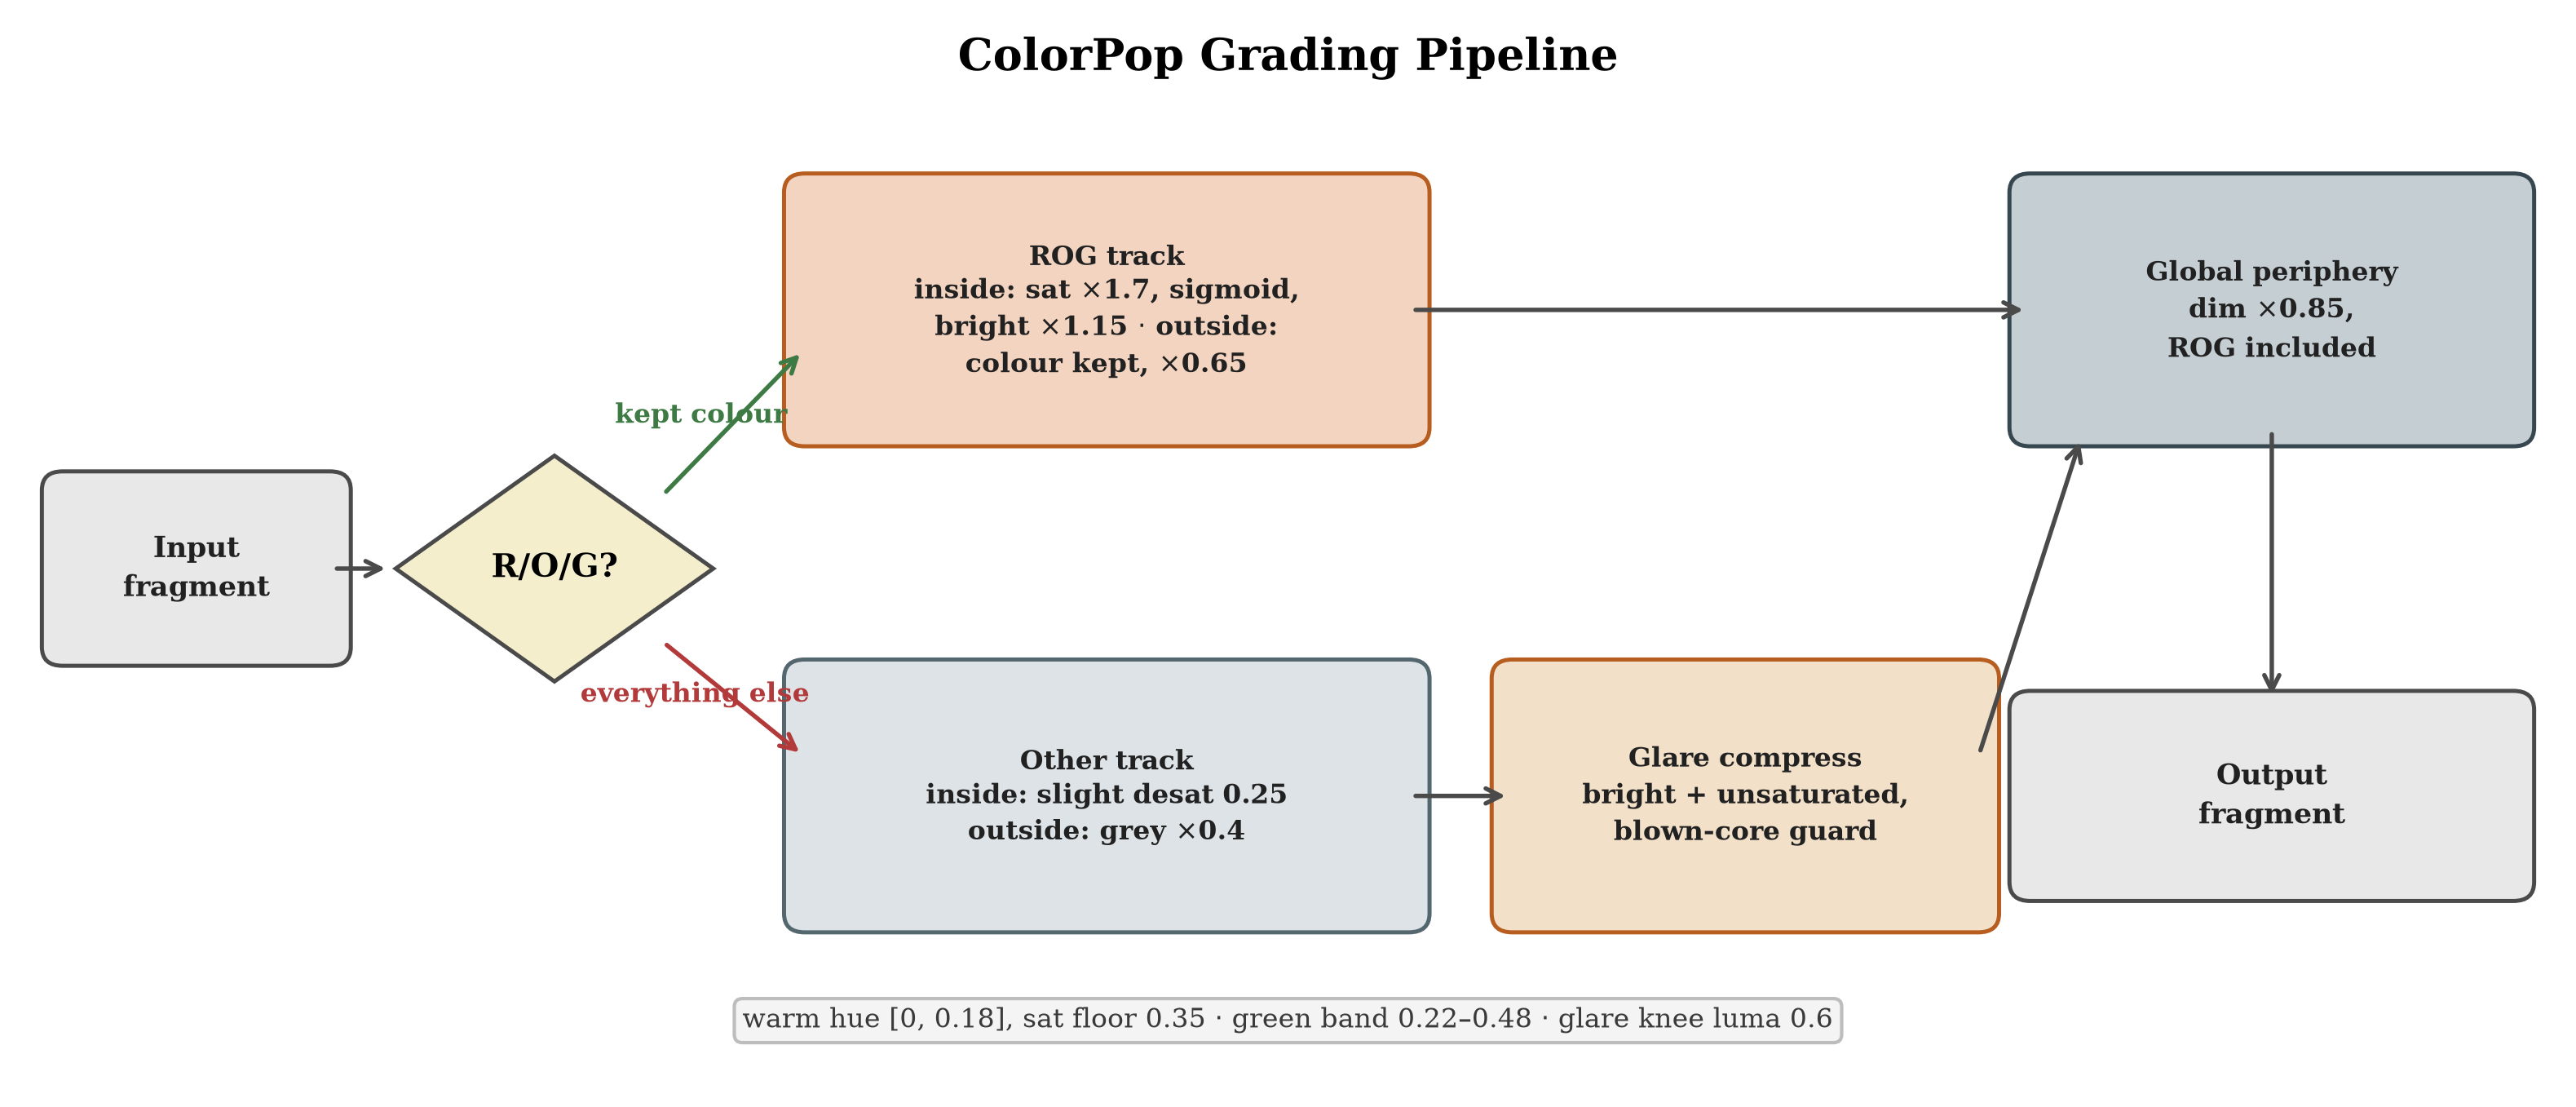
\includegraphics[width=\linewidth]{content/figures/fig_colorpop_pipeline.png}
\caption{ColorPop grading pipeline flowchart.}
\label{fig:colorpop}
\end{figure}

\subsection{The superseded and exploratory family}

Six further modes are retained in shader and enumeration but excluded from evaluation.
Table~\ref{tab:modes} gives each with the source it derives from and the reason it was not carried
forward. Each is reported as an explored design point carrying no evaluation claim.
Figure~\ref{fig:modefamily} shows nine of the ten peripheral treatments as captured on device,

\begin{figure}[htbp]
\centering
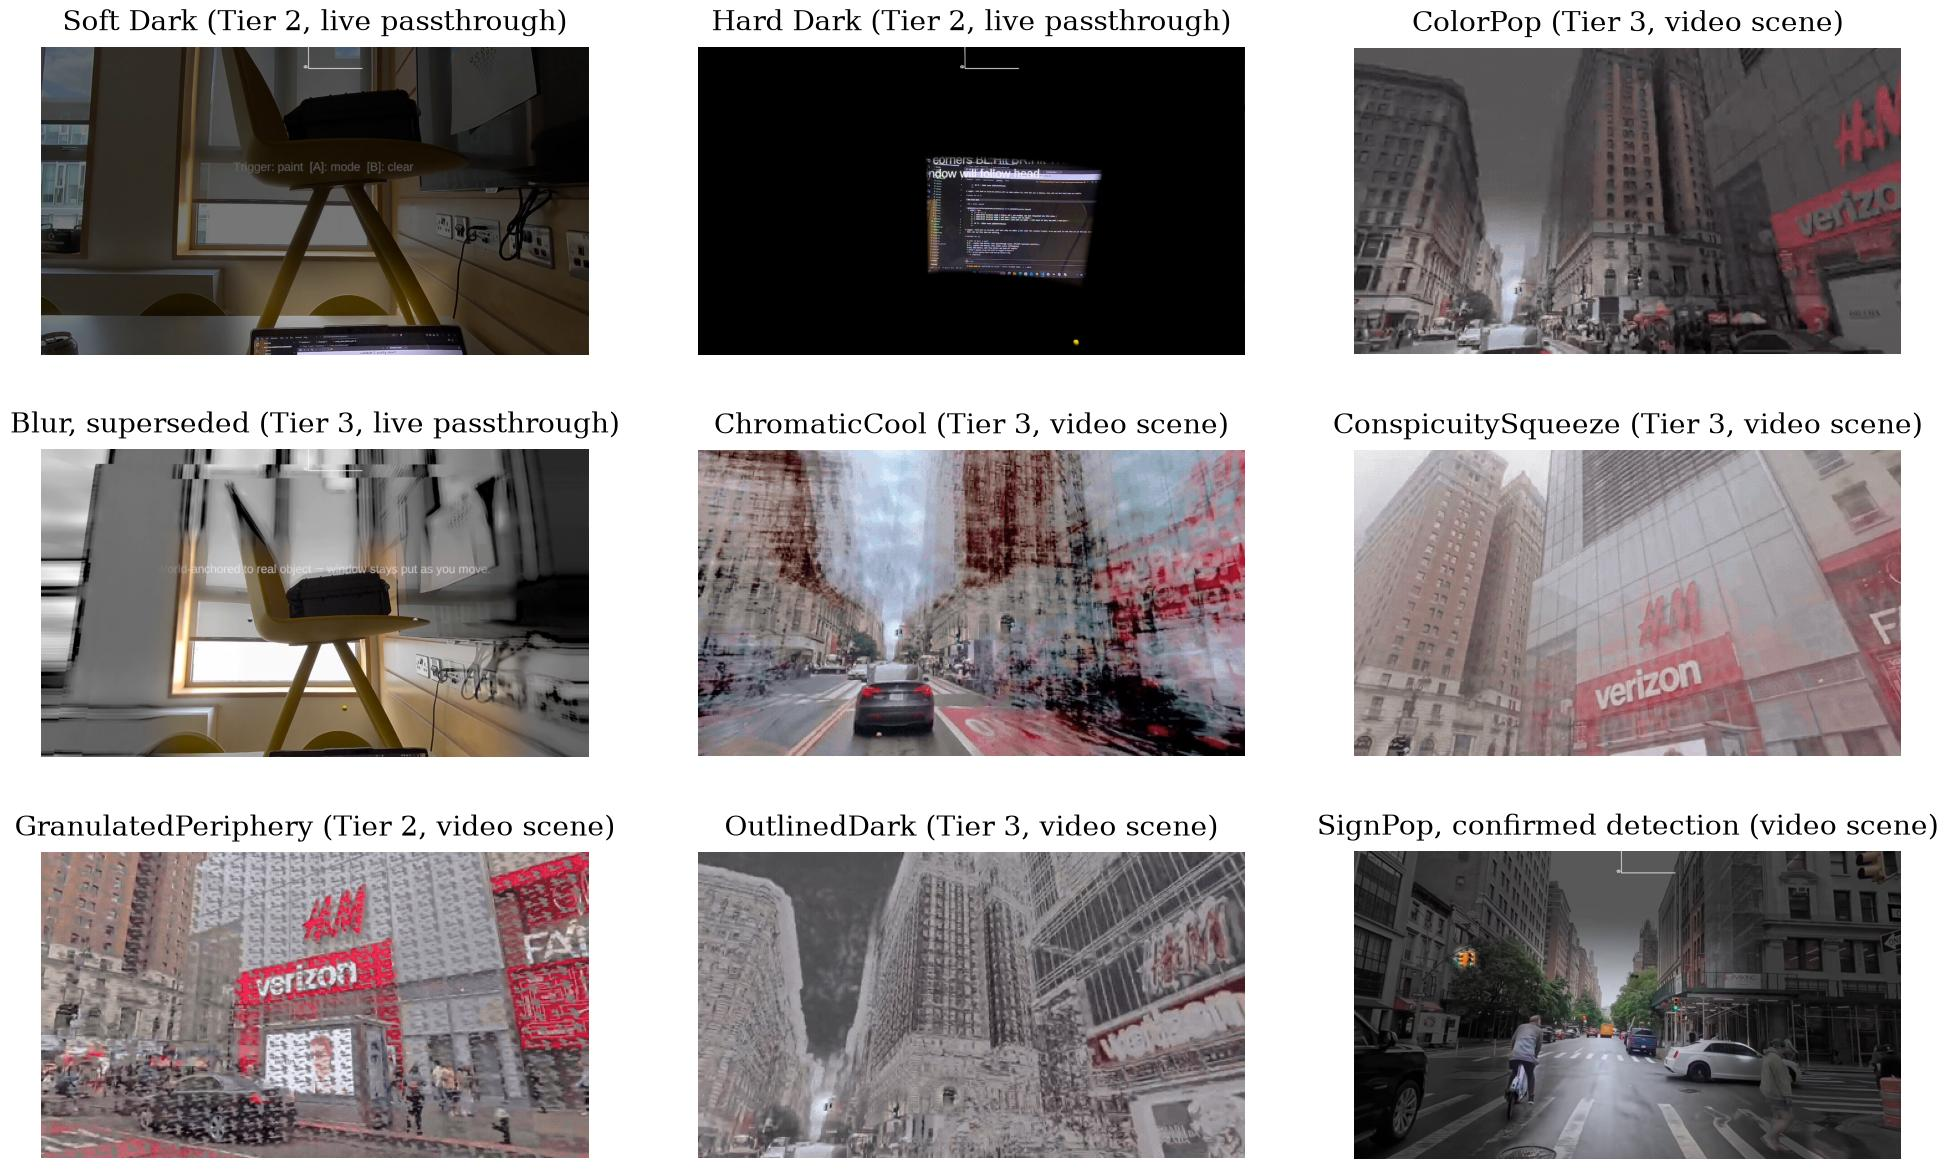
\includegraphics[width=\linewidth]{content/figures/fig_mode_family.jpg}
\caption{Nine of the ten peripheral treatments, from on-device recordings. The passthrough captures
show the world-locked window revealing untouched passthrough; the video-scene captures show
full-field grading over the driving clip. Blur's contrast-restoration pass reads as an edge drawing
rather than a smooth defocus, one reason it was superseded. SpotLift is not shown: it exists only on
the video path and no recording of it was retained. TintedDark is dead code.}
\label{fig:modefamily}
\end{figure}

\begin{longtable}{p{0.20\textwidth}|p{0.38\textwidth}|p{0.28\textwidth}}
\caption{Modes built but not evaluated, with the source each derives from and the reason it was not
carried forward.}
\label{tab:modes} \\
\hline
\textbf{Mode} & \textbf{What it does} & \textbf{Why not evaluated} \\
\hline
\endfirsthead
\hline
\textbf{Mode} & \textbf{What it does} & \textbf{Why not evaluated} \\
\hline
\endhead
\hline
\textbf{Blur} (superseded) & Progressive Gaussian blur of the camera periphery with delayed desaturation, a perceptual noise term after \citet{tariq2022}, and contrast restoration after \citet{patney2016} & Whole-periphery blur was the least subtle of five methods and irritated 59 of 102 participants in its own source study \citep{grogorick2018}. Also the heaviest shader path in the family \\
\textbf{ChromaticCool} & Warm window against a cool periphery, chromatic opposition & Luminance modulation outperforms warm–cool chromatic modulation in its own source study \citep{bailey2009} \\
\textbf{Conspicuity\-Squeeze} & Centre–surround contrast flattened toward the local mean, after \citet{veas2011} & Brightened the periphery instead of squeezing its contrast, the opposite of the intent, confirmed by shader inspection \\
\textbf{Granulated\-Periphery} & World-locked static noise grains with eccentricity-ramped density, after \citet{cao2021} & Grains occlude fine detail, the wrong failure mode for a driving scene where the detail is the target \\
\textbf{OutlinedDark} & Near-blackout with luminance edges restored, following the finding of \citet{cheng2022} that context-preserving outlines reduce anxiety & Surviving edges read as a comic-book style that early testers found more interesting than the task \\
\textbf{SpotLift} & Focus-region brightness lift over a soft peripheral dim & Cannot exist on the passthrough path at all, since OS passthrough cannot be brightened. Video path only \\
\hline
\end{longtable}

A seventh candidate, \textbf{TintedDark}, a configurable-colour overlay, is dead code. It has no
proposing paper and no mechanism the dark family does not already have. Its shader branch and enum
entry remain only because removing the entry would break a serialized scene value (Section 4.10).

One sampling detail from the Blur path generalises to any equirectangular source: taps must wrap
horizontally for a seamless 360$^{\circ}$ join and fold back rather than clamp vertically, since
clamping smears the top and bottom texture rows across the sky and floor, and the tap radius must
fade toward the poles, where any UV-space offset corresponds to a huge angular distance.

\subsection{Cost structure of the shader paths}

The mode family spans roughly two orders of magnitude in per-fragment cost, and the gradient is
structural rather than incidental. It is Chapter 3's deployability axis realised in instructions. The
dark modes take an early return after the window test: no texture reads, a handful of arithmetic
operations, one blended write. ColorPop reads the source texture once per fragment on its main path,
plus a 17-tap Gaussian surround only in the small fraction of fragments where the glare mask fires
with the core guard enabled, and its cost is dominated by per-pixel colour arithmetic. The Blur path
is the heaviest: two Gaussian rings of eight taps each around a shared centre per camera, doubled
when both cameras are live near the stitch, plus the noise texture read and contrast-restoration
arithmetic.

These per-fragment counts are structural, and Section 4.11 confirms the gradient they predict with
measured frame times: the dark modes cost nothing measurable over an empty passthrough scene, and
the heaviest camera path costs roughly two and a half times the dark modes' frame time while still
holding the display's frame rate. The design consequence stands in both the structure and the
measurement: the modes the study asks participants to imagine using for long sessions, the dark
family, are the modes that cost almost nothing, and the mode with the richest effect is the one
whose Tier-3 pipeline carries the platform's thermal ceiling.

\begin{figure}[htbp]
\centering
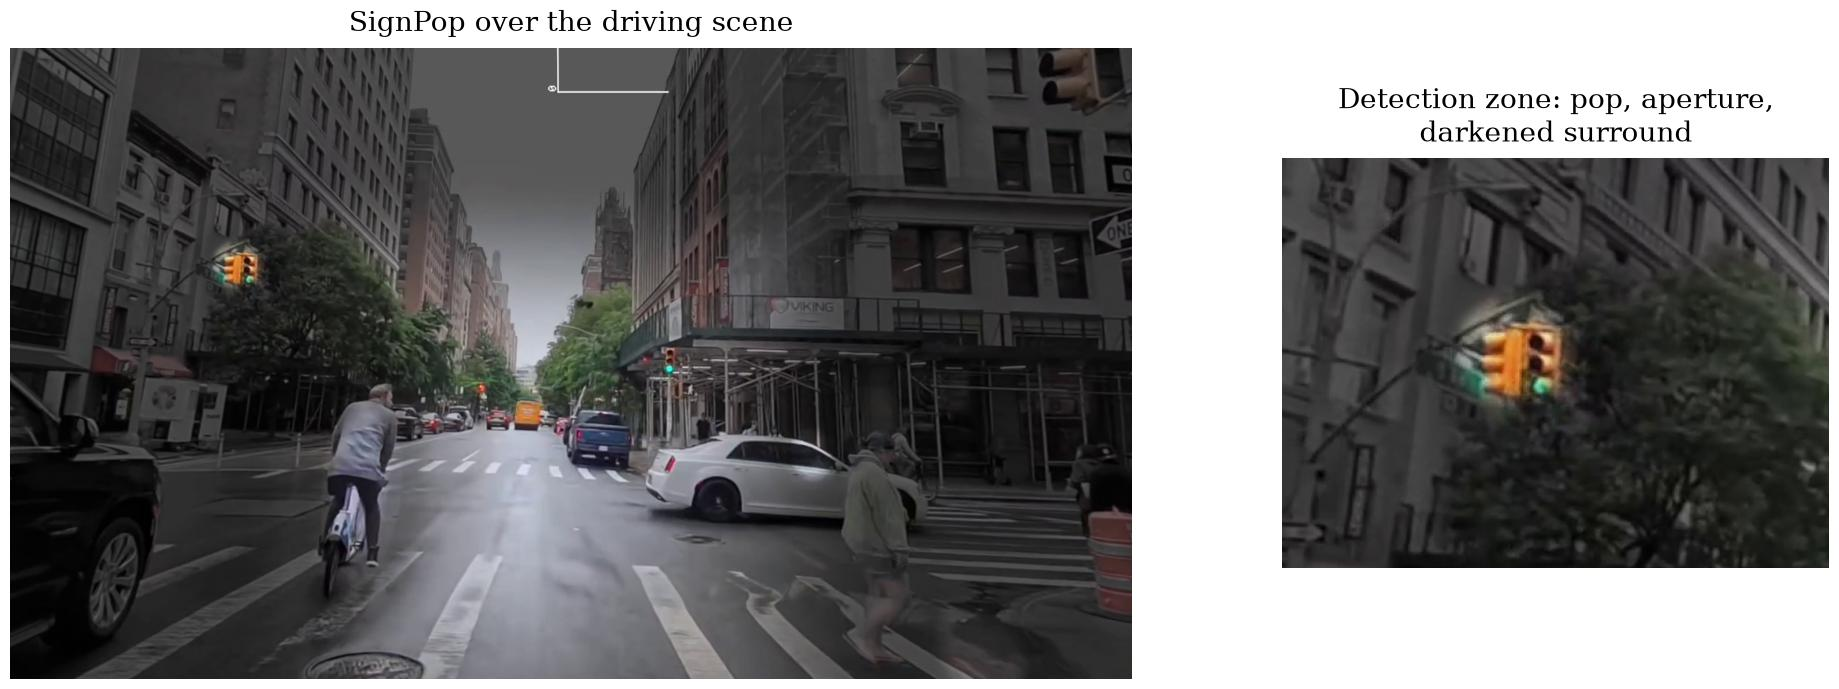
\includegraphics[width=\linewidth]{content/figures/fig_signpop_photo.jpg}
\caption{SignPop over the driving scene, from an on-device recording. Non-signal content is graded
to dim grey, kept red--orange--green pixels stay visible everywhere, and a confirmed detection
(right, enlarged) fires the full bundle: colour pop, detection aperture, saliency lift, and darkened
surround.}
\label{fig:signpopphoto}
\end{figure}

\subsection{Detection-gated salience re-grading (SignPop)}

\textbf{SignPop} is the most capable of the ten peripheral treatments, live only in the video test
scene, and it is the mode placed in
front of participants in the driving block (Figure~\ref{fig:signpopphoto}). It shares ColorPop's
four-level ROG grading pipeline, but
a confirmed detection from the offline oracle track (Section 4.8) gates a bundle of effects rather
than colour alone.

\textbf{The colour gate.} ColorPop already keeps ROG hues partly visible in the periphery without any
detection. SignPop restricts the \textit{full} vivid treatment to pixels inside a confirmed detected
box. An undetected ROG pixel, whether neon signage, brake lights, advertising, or a genuine bake
miss, falls back to a partial keep (default 0.35) rather than full grey, a graceful miss so a missed
real signal is dimmed rather than hidden. A short hold of 0.5 s keeps a detection alive after it
drops out of the bake, so pops do not blink between samples taken every half second.

\textbf{An independent detection-zone system.} Beyond the colour gate, every confirmed detection
drives three further, colour-independent effects computed from soft elliptical zones around each
detection box. A \textbf{detection aperture} carves the vignette away directly over the object. This
is not the focus window of Section 4.2: it is a separate, transient opening appearing wherever a
detection is confirmed, inside or outside the focus window, and disappearing when the detection is
lost. A \textbf{saliency lift} boosts saturation, brightness, and local contrast around the object,
at full strength when the object sits inside the focus window and scaled down outside it, since in
the periphery the aperture has already opened a clear region around the object and the additional
pop only needs to be subtle. A
\textbf{darkened surround} dims a soft annulus just outside the object's boundary, raising the
object's centre–surround contrast from both sides, after the dual modulation of \citet{veas2011}. The
saliency lift additionally oscillates at approximately 1 Hz, following \citet{waldner2014} on
low-frequency, low-amplitude temporal modulation attracting attention with low annoyance, far below
the 15–25 Hz photosensitivity band.

This entire detection-zone system is suppressed for Hard Dark. Once the user-placed window is locked,
no detected object anywhere gets a carve-out, however salient. This is a deliberate choice rather
than an omission: Hard Dark's role is to test the strongest possible manipulation, full occlusion
with no exceptions, against a workstation task with no peripheral object the participant needs to
see. Adding detection apertures back into Hard Dark would weaken exactly the property the
confirmatory test relies on. A detection-aware variant is a reasonable extension for contexts where a
peripheral object genuinely matters, and the conclusion returns to it as future work.

\textbf{Gates on what counts as a detection at all.} The offline bake considers only the forward
view, azimuth $\pm$90\textdegree{} and elevation $\pm$50\textdegree{} around video-centre,
so a detection behind the participant never enters the track. At runtime, apparent size then decides
whether a detection is allowed to draw anything, and the two target classes are gated separately
because they fail in different ways.

For signals, the gate is on the larger of the box's angular extents and is set to
1.0\textdegree{} in the driving scene. Of the 203 post-debounce traffic-light lifetimes in the
deployed track, 19 never clear it, so a distant light does not open a window over what is still,
perceptually, a speck. For people the concern is not resolvability but relevance and volume, so they
bypass that gate and take a higher threshold on box \textit{height} of 3\textdegree{}, which for a
1.7 m adult corresponds to roughly 32 m, combined with the positional gate of Section 4.8.1. A
pedestrian far enough away to be irrelevant to the next few seconds of driving is therefore silent
even though the box is comfortably large enough to render.

\textbf{What a confirmed detection actually switches on.} Six effects fire together on the same gate:
the colour-pop upgrade, the window carve-out, the saturation lift, the brightness lift, the contrast
expansion, and the darkened surround, layered on the $\sim$1 Hz pulse. \textbf{None of the six is
isolable in the current build.} This is the single most important limitation on what any measured
effect can be attributed to, and it is stated here, where the mechanism is, rather than repeated
wherever a result appears. The conclusion proposes the three-arm design that would separate them.

\section{Motion-Based Suppression}

Head-coupled restriction of the visual field is a known comfort hazard: \citet{norouzi2018} found
that vignetting yoked to head rotation \textit{increased} rather than decreased simulator sickness.
The system therefore decouples in the opposite direction. The effect \textbf{fades out while the head
moves fast, and returns when it settles.}

Each frame the manager computes head angular speed between successive head rotations. When speed
exceeds a per-mode threshold, a suppression scalar animates toward 1 over 0.20 s, and once speed has
stayed below threshold for the mode's hold time, back toward 0 over 0.70 s. Thresholds and holds
scale with the mode's intrusiveness: Blur 30$^{\circ}$/s with a 0.6 s hold, ColorPop 35$^{\circ}$/s
with 0.7 s, Soft Dark 50$^{\circ}$/s with 1.0 s, Hard Dark 70$^{\circ}$/s with 1.5 s. The blackout
mode tolerates the most motion before yielding and waits longest before returning, because wrongly
suppressing a strong effect flashes the whole periphery back into view, while wrongly suppressing a
gentle one costs little. The fade asymmetry follows the same logic: yielding should feel immediate
to be trusted, and returning can be slower because little is at stake.

The shader receives \verb|effectiveStrength = m_vignetteStrength * (1 - suppression)|, so suppression
multiplies the formation state rather than resetting it, and a glance over the shoulder during the
three-second formation does not restart the transition. State the user created, the locked window and
the accumulated formation, is never destroyed by a comfort mechanism, only veiled.

One refinement matters for the interaction loop. If the head's direction enters the focus window,
with a $+$15$^{\circ}$ margin, the hold timer is zeroed immediately, so arriving back at the focus
region restores the effect at once. The asymmetry is deliberate. Looking \textit{away} is treated as
a possible need for situational awareness, so the effect yields generously, while looking \textit{back
at the task} is treated as re-engagement, so it returns promptly. Figure~\ref{fig:suppression} shows
the threshold, the hold timer, the two fade ramps, and the focus-arrival shortcut as one state
diagram.

\begin{figure}[htbp]
\centering
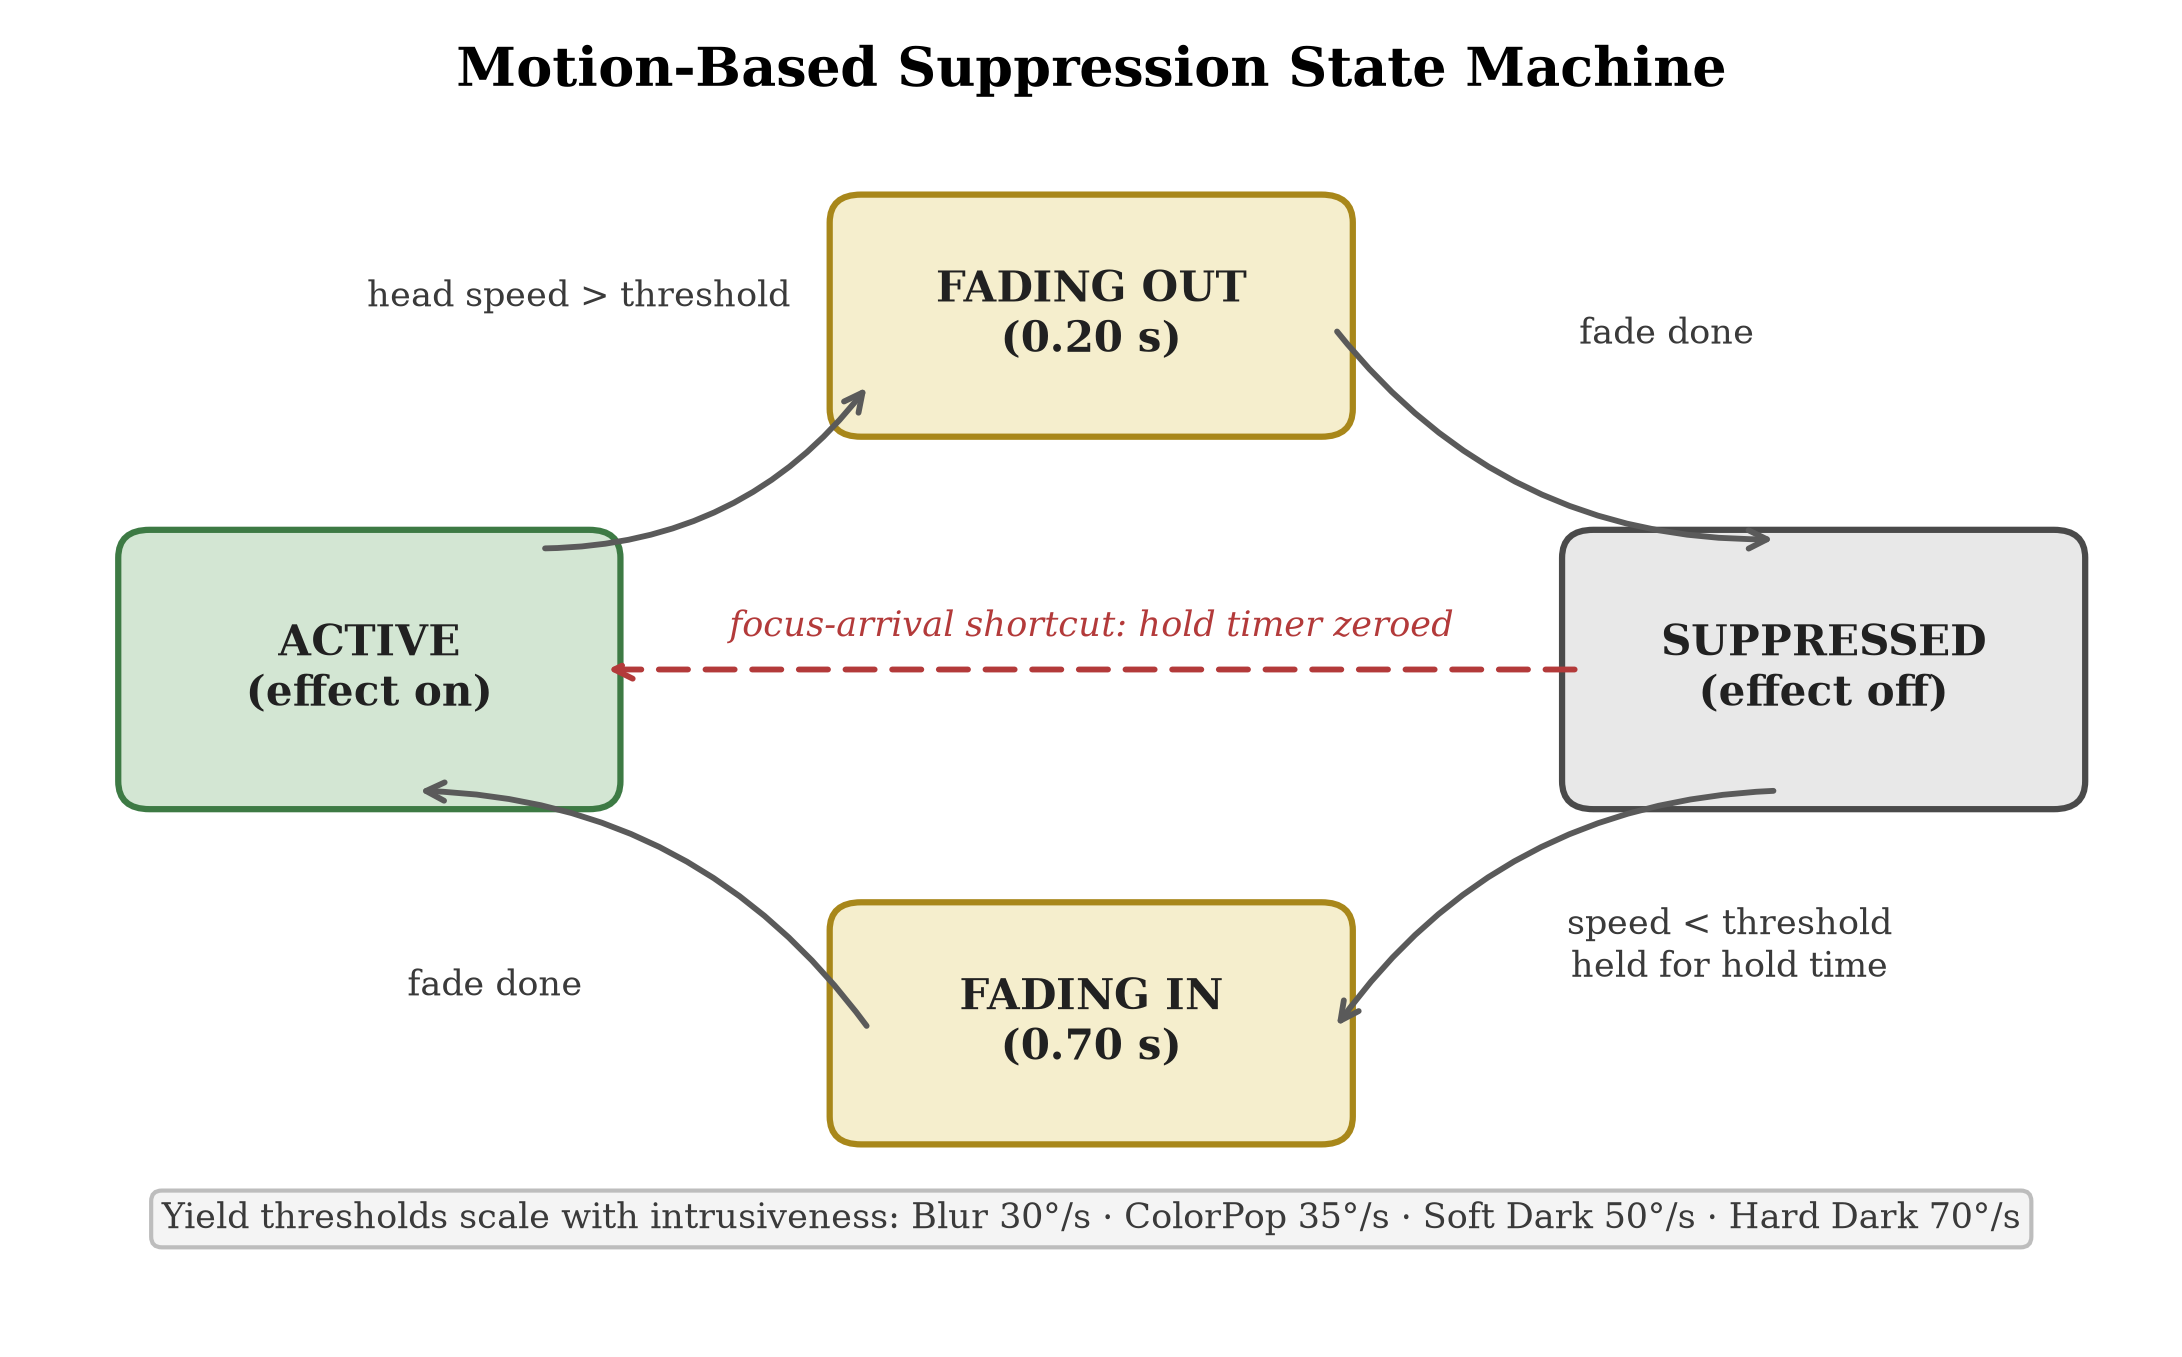
\includegraphics[width=\linewidth]{content/figures/fig_motion_suppression.png}
\caption{Motion-based suppression: speed threshold, hold timer, and fade ramps.}
\label{fig:suppression}
\end{figure}

\section{Interaction Design}

The user defines the focus window by \textbf{painting} it. Holding the right controller trigger
sweeps the controller's aim across the scene, and the window rectangle grows to enclose the swept
region, seeded at the aim point with a small brush pad. Releasing the trigger \textbf{locks} the
window and, in the dark modes, starts the three-second formation. The rectangle is computed and
stored directly in the world azimuth and elevation coordinates of Section 4.2.2, so what the user
paints is what stays locked to the room. The A button cycles modes and B clears the window.

Feedback is deliberately minimal. Five dot markers, four corners plus an aim cursor, show the window
during painting, dim on lock, and auto-hide after three seconds. A world-space toast announces mode
changes and fades away. Hand tracking is disabled and input is controller-only, a scope decision that
removes a class of input ambiguity from the study sessions.

Three design rationales are worth making explicit. \textit{Painting rather than pointing}: a focus
window is a region rather than a point, and sweeping it makes the region's extent a deliberate act,
where auto-sizing a window around a pointed target would hide a consequential parameter inside a
heuristic. \textit{World-locking rather than head-locking}: the window belongs to the task surface
rather than the gaze, and a head-locked window would chase attention rather than anchor it, which is
also the comfort hazard Section 4.6 exists to avoid. \textit{Formation as transition}: the ramp
exists because an instantaneous peripheral blackout would be startling, and it doubles as the user's
confirmation that the lock succeeded. Figure~\ref{fig:interaction} follows one placement from
painting to locked formation.

\begin{figure}[htbp]
\centering
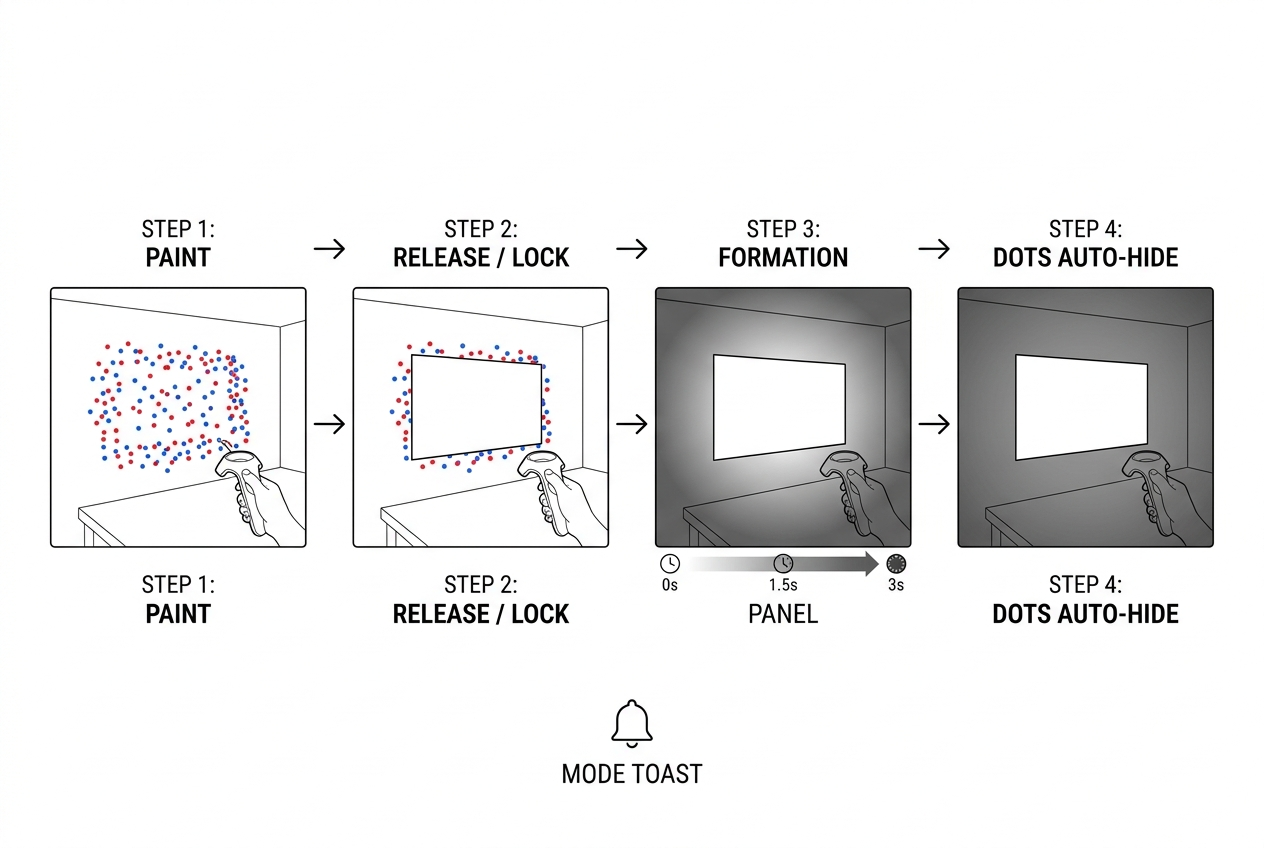
\includegraphics[width=\linewidth]{content/figures/fig_interaction_sequence.jpg}
\caption{Interaction sequence for placing and locking the focus window.}
\label{fig:interaction}
\end{figure}

\section{Perception: Detection Islands and the Offline Oracle}

\subsection{Live detection support}

The live passthrough manager supports up to eight simultaneous \textbf{detection islands}, azimuth
and elevation rectangles fed by an optional \verb|YoloRunner| component, inside which the vignette is
cleared so the detected object shows through undiminished. Each island renders as a soft-edged
ellipse with the dual modulation after \citet{veas2011} described in Section 4.5.5. Detections expire
after 0.6 s without renewal. Its class filter is deliberately narrow, COCO classes 9 (traffic light)
and 11 (stop sign) only, with people excluded because a crowded street would otherwise fill every
aperture slot with pedestrians.

The evaluated driving block runs from the baked track instead, for the oracle-perception reason set
out in Section 4.8.2, so its admitted classes are the baked ones: traffic lights and people. People
there carry an additional positional gate, since a driving scene contains far more pedestrians than
the sixteen-slot budget can hold and most are not safety-relevant. A person is highlighted when they
fall inside the focus window, or when they sit within 22.5$^{\circ}$ of its boundary, with that
acceptance widening in proportion to apparent size so that a pedestrian the car is approaching stays
highlighted as they pass out of the window rather than being dropped at their nearest moment.

Two properties of the aperture system are stated here because they bound what it can do in a crowded
scene. First, the caps above are a hard budget: the live path holds eight simultaneous apertures and
the video path sixteen, slots fill in the order detections arrive, and any detection beyond the cap
is dropped. There is a budget but no prioritisation, so a crowded scene degrades by dropping the
newest detection rather than the least important one. Neither cap was reached in any reported
session, but that is a property of the study footage rather than a design guarantee. Second, a
detection is characterised only by its angular position and apparent size, evaluated per frame with
the minimum-lifetime gate and smoothing fades described below. There is no velocity or trajectory
term anywhere in either path, so a pedestrian stepping off a kerb and one standing still receive
identical treatment if they subtend the same angle. Both limits are carried into Chapter 6.

\subsection{The offline oracle pipeline}

For evaluation, live inference is replaced by a \textbf{pre-baked detection track}. This is the
oracle-perception commitment named in Chapter 1: the study asks whether an effect built on excellent
detection helps attention, without first building excellent detection on-device. A PC-side script
(\verb|Tools/bake_detections.py|) runs YOLO11 \citep{jocher2024} over the full-resolution
5760$\times$2880 study video. Each sample takes the forward crop of the equirectangular frame,
$\pm$90$^{\circ}$ in azimuth and $\pm$50$^{\circ}$ in elevation, and runs it as 4$\times$3
overlapping tiles plus a pass over the whole crop, thirteen inferences per sample, merged by
per-class non-maximum suppression. Sampling is at 0.5 s intervals, and the script writes a JSON
track keyed by video time. The runtime loads it and plays detections back deterministically.

Full resolution is the point rather than an indulgence. Detections that serve as ground truth or as
pre-scripted salience input must be computed at a resolution the live pipeline cannot afford, which
is exactly what makes them an \textit{oracle}. Distant traffic lights are the binding case: they are
fully visible to a human viewer but subtend few pixels, so they fall below detectable size in a
downsampled frame.

The raw bake detects every traffic light and sign in the forward crop, including many that do not
govern the driver's lane: cross-street and pedestrian-facing signals, signals turned away from the
camera, and unrelated distant lights. Since the runtime has no relevance filtering of its own and
SignPop would highlight all of them equally, a curation pass
(\verb|Tools/triage_traffic_lights.py|) reconstructs each real-world signal's lifetime using the same
identity heuristic as the runtime tracker, buckets it by azimuth from video-forward, and moves the
lane-irrelevant ones into a sidecar file. Roughly 1,300 detections were set aside this way. The
sidecars are kept alongside the deployed track, so the split is inspectable and fully reversible.

\textbf{The deployed track over the 8-minute-39-second study clip holds 13,939 detections across
1,040 sampled frames, with 99.5\% of sampled frames containing at least one detection} (median 14 per
sample; 2,952 traffic lights and 10,987 people). Two properties matter for the rest of the
dissertation. First, it confirms the footage is genuinely event-dense, a precondition for its role as
the driving-block stimulus. Second, it fixes a versioned detection set that the study's stimuli are
read from directly, so those stimuli are artifacts rather than descriptions. Reproducing the track
from source requires the bake and the curation step together, both of which are in the repository.

What the bake does \textit{not} establish is equally important. It says nothing about on-device
feasibility, and nothing about detection quality in absolute terms, since full-resolution YOLO11 is a
\textit{reference} rather than truth verified against human annotation. The gap between this oracle
and a live on-device detector was never measured. Every statement in this dissertation about
detector-dependent guidance is therefore conditioned on oracle-quality detection, and the conclusion
carries closing that gap as the first item of future work. Unlike the live manager, the video scene's
manager draws on the shader's full sixteen-slot detection array, which absorbs the bake's density, so
no ordering or survival policy is needed for the great majority of samples.
Figure~\ref{fig:oracle} shows the pipeline from source video to deterministic playback.

\begin{figure}[htbp]
\centering
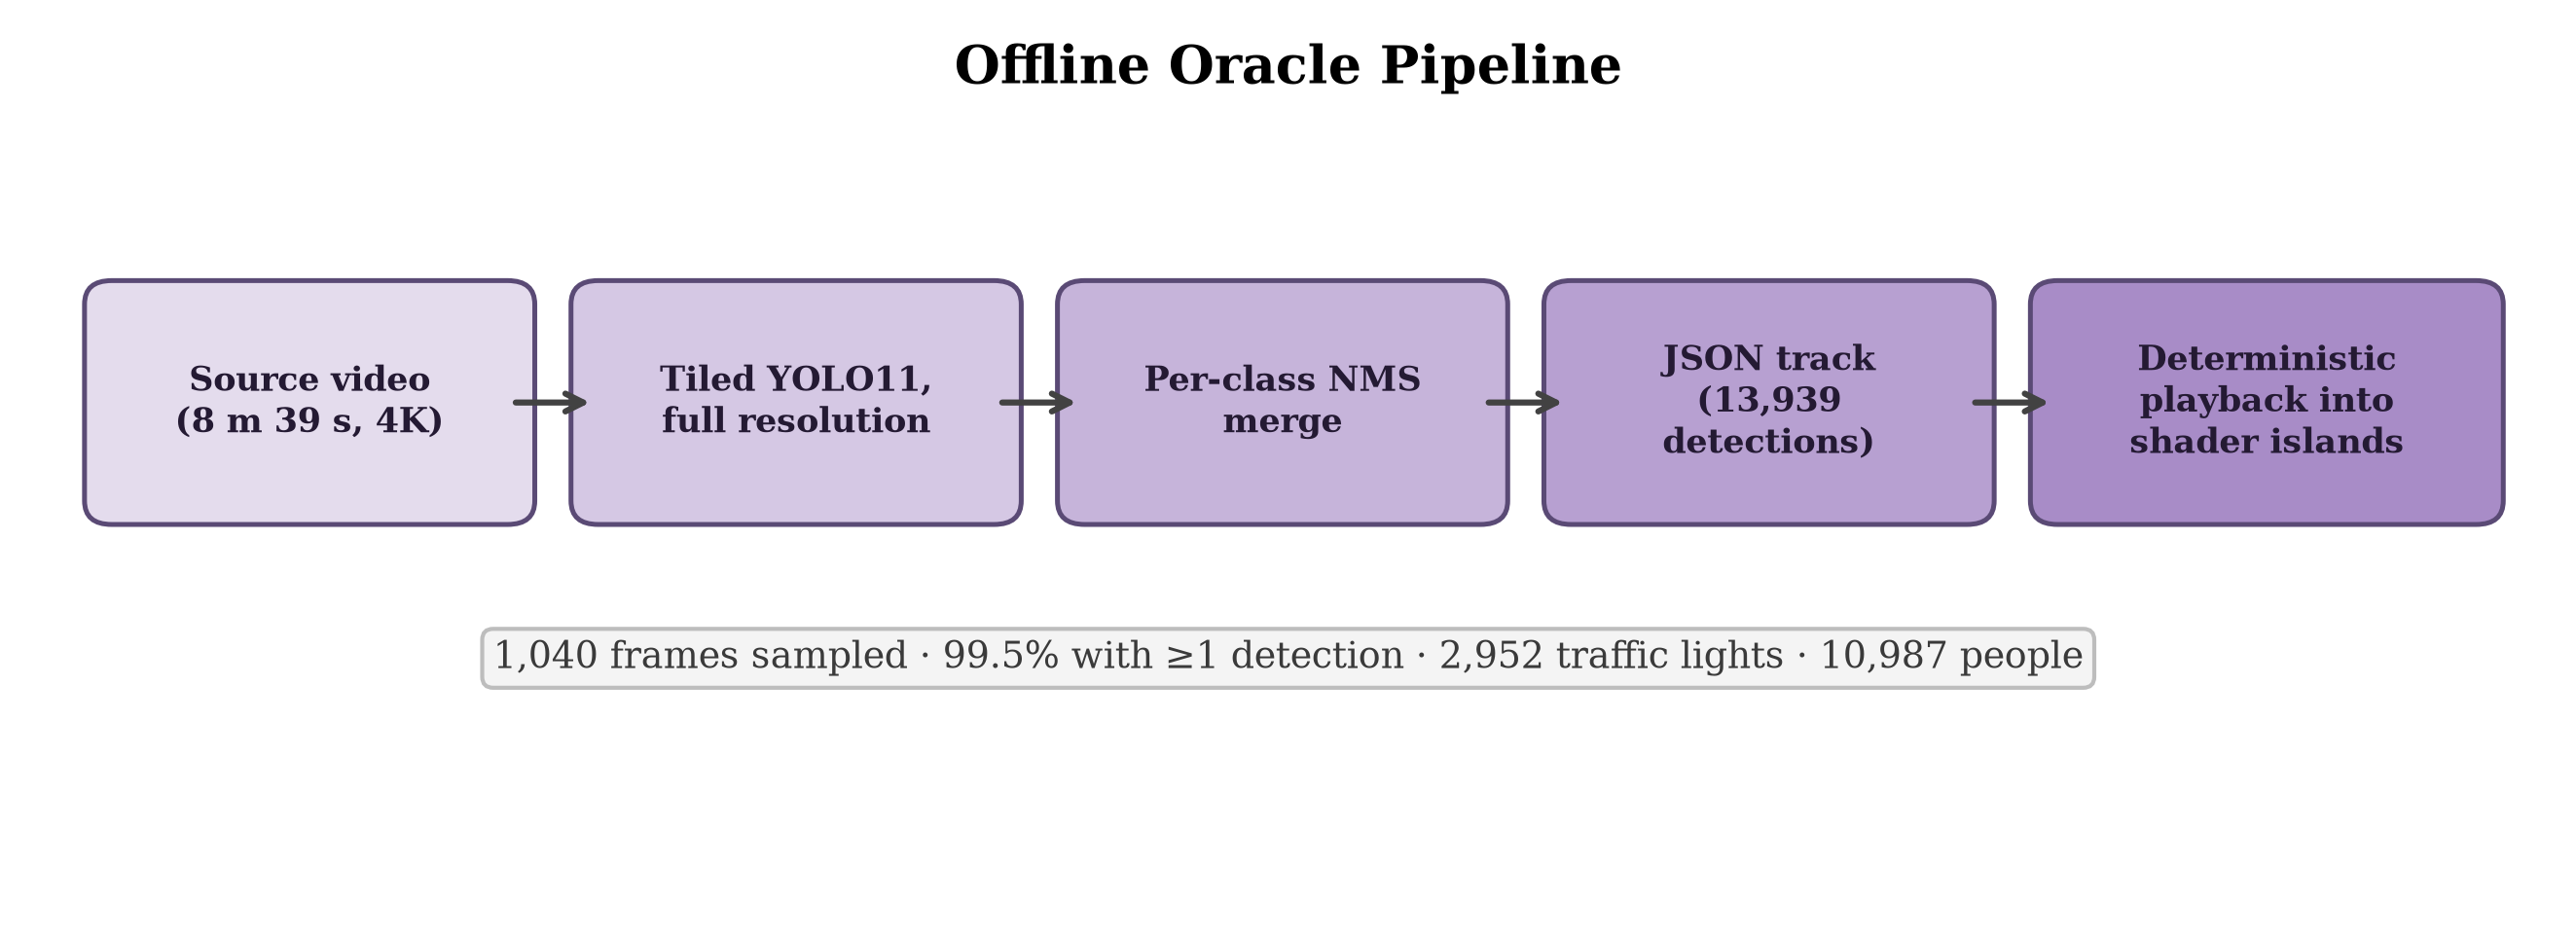
\includegraphics[width=\linewidth]{content/figures/fig_oracle_pipeline.png}
\caption{The offline oracle pipeline, from source video to deterministic playback.}
\label{fig:oracle}
\end{figure}

\section{The Video Test Scene}

All dynamic-scenario evaluation runs in a dedicated harness scene in which the passthrough layers are
replaced by an 8-minute-39-second equirectangular driving clip decoded onto the sphere. The scene
preserves everything else, the same shader, window logic, modes, interaction, and detection islands,
so a mode behaves identically over video and over the live camera feed, while gaining what live
passthrough can never provide: \textbf{identical, repeatable, event-dense stimuli for every
participant}, plus a deterministic ground-truth detection track. The harness is thus the
simulation-based evaluation instrument of Chapter 5's driving block.

The equirectangular mapping exposes UV offsets and a vertical flip so any source clip's forward
direction and horizon can be registered without re-encoding the video, and a live-inference path
maintains a dedicated downsampled render target for the detector via Unity Sentis \citep{unity2024}
so it never reads the 4K texture directly. For evaluation that path is bypassed in favour of the
baked track.

Two harness-specific notes have study consequences. In the video scene SignPop's grading covers the
full sphere including the window, which is the intended driving-block configuration. And the video
manager's motion-suppression master switch defaults to \textbf{false} while the driving block
specifies suppression active, so the session sequencer asserts the required configuration at start-up
rather than leaving it to the scene's saved state.

\section{The Failure Museum}

This section reports the failures that shaped the system, on the view that documented dead ends are
reusable knowledge: each with what was tried, why it failed, and what replaced it.

\textbf{1. Screen-space camera sampling $\rightarrow$ double vision.} The first shader sampled the
camera texture by screen position. Per-eye the image was correct. Binocularly it could not fuse,
because each eye sampled a different camera pixel for the same world point. The on-device symptom was
frank double vision. Replaced by world-direction sampling through a head-centred pinhole
(Section 4.4), verified fused on device. Lesson: in stereo rendering, eye-independence of the
sampling domain is a correctness criterion, not an optimisation.

\textbf{2. Surface-projected passthrough $\rightarrow$ deprecated API.} The obvious platform
mechanism for putting real passthrough on application geometry was evaluated and rejected because it
is deprecated as of SDK v83. Any architecture built on it would be built on removed ground. Replaced
by the window-as-absence composite, which uses only stable compositor behaviour. Lesson: on young
platforms, prefer primitives the OS must keep, such as alpha compositing, over conveniences it may
withdraw.

\textbf{3.} \verb|Shader.Find| \textbf{on device $\rightarrow$ null.} Runtime materials created by looking a
built-in shader up by name worked in the editor and silently returned null on Quest, because Android
builds strip shaders that no serialized asset references, and the failure surfaced as a crashed
startup coroutine rather than an error. Replaced by a serialized template material that
runtime dots clone, since the asset reference guarantees build inclusion. Lesson: never construct
device materials from name lookups. Ship a serialized template.

\textbf{4. Downsampled detection baking $\rightarrow$ missing traffic lights.} The first oracle bake
ran YOLO on a 640$\times$360 downsample of the 4K source. Distant traffic lights fell below detectable
pixel size and the track silently omitted most of them, an oracle that was not an oracle. Replaced by
the full-resolution tiled baker of Section 4.8.2, raising coverage to 99.5\% of samples. Lesson:
validate ground-truth pipelines against the \textit{smallest} objects they must contain, and never
let the convenience path overwrite the reference track.

\textbf{5. Two operational traps, recorded for the protocol rather than the architecture.} The
platform's camera-based screenshot service returns black frames whenever the application holds the
passthrough camera, because the two contend for the same resource, so the study's redundant session
recording must use framebuffer capture instead. And the headset sometimes boots with controllers in
\verb|CONNECTED_INACTIVE|, leaving the application with no input at all and no way to distinguish
that from a broken build, so the study build boots straight into the experiment scene, hand tracking
is disabled, and waking the controllers is a line on the pre-session checklist. Lesson: input
liveness is an environmental precondition, so it belongs in the protocol rather than the debugger.

\section{Technical Validation: Frame Cost and Legibility}
\label{sec:techval}

Two claims have carried this chapter so far on structural argument alone: that the camera-free dark
modes are cheap enough to deploy for long sessions, and that the native passthrough served through
the window is visibly better than the Tier-3 camera re-render it spares the user from. Both were
measured on the study hardware on 7 August 2026, against criteria fixed before the data was seen.

\subsection{Per-mode frame cost}

Frame cost was captured with the platform's OVR Metrics Tool, which logs one row per second of the
application's GPU frame time, stale-frame count, and per-core CPU and GPU utilisation. One
continuous run in the passthrough scene stepped through effects off, Soft Dark, Hard Dark and Blur,
and a second run in the video scene covered SignPop and effects off, with every switch logged
against the wall clock. Five seconds are trimmed from both ends of each segment so formation
transitions do not contaminate a segment's statistics, leaving 79 to 245 samples per configuration.
The pre-stated pass criterion for the study configurations is a 95th-percentile GPU frame time
within the 13.88 ms budget of the 72 Hz display and a stale-frame rate below 1\%. Blur was
pre-stated as an interpretation band rather than pass/fail, since its cost relative to Soft Dark is
the price of Tier-3 camera re-rendering either way. Table~\ref{tab:t1} gives the results and
Figure~\ref{fig:t1} plots them against the budget; the analysis script and raw captures are in the
project record.

\begin{longtable}{p{0.26\textwidth}|p{0.10\textwidth}|p{0.10\textwidth}|p{0.10\textwidth}|p{0.12\textwidth}|p{0.10\textwidth}}
\caption{Per-mode frame cost from the OVR Metrics captures. GPU times are the application's own
frame time in milliseconds against the 13.88 ms budget; stale rate is stale frames as a share of
display frames; CPU is the worst core's mean utilisation.}
\label{tab:t1} \\
\hline
\textbf{Configuration} & \textbf{GPU p50} & \textbf{GPU p95} & \textbf{Stale} & \textbf{CPU worst} & \textbf{GPU util} \\
\hline
\endfirsthead
\hline
\textbf{Configuration} & \textbf{GPU p50} & \textbf{GPU p95} & \textbf{Stale} & \textbf{CPU worst} & \textbf{GPU util} \\
\hline
\endhead
\hline
Effects off (passthrough) & 3.23 & 3.37 & 0.30\% & 68\% & 41\% \\
Soft Dark & 3.25 & 3.34 & 0.00\% & 62\% & 41\% \\
Hard Dark & 3.17 & 3.32 & 0.02\% & 61\% & 41\% \\
Blur & 8.01 & 8.15 & 0.09\% & 63\% & 79\% \\
SignPop (video scene) & 8.62 & 11.42 & 7.29\% & 48\% & 71\% \\
Effects off (video scene) & 10.07 & 12.36 & 7.89\% & 49\% & 79\% \\
\hline
\end{longtable}

\begin{figure}[htbp]
\centering
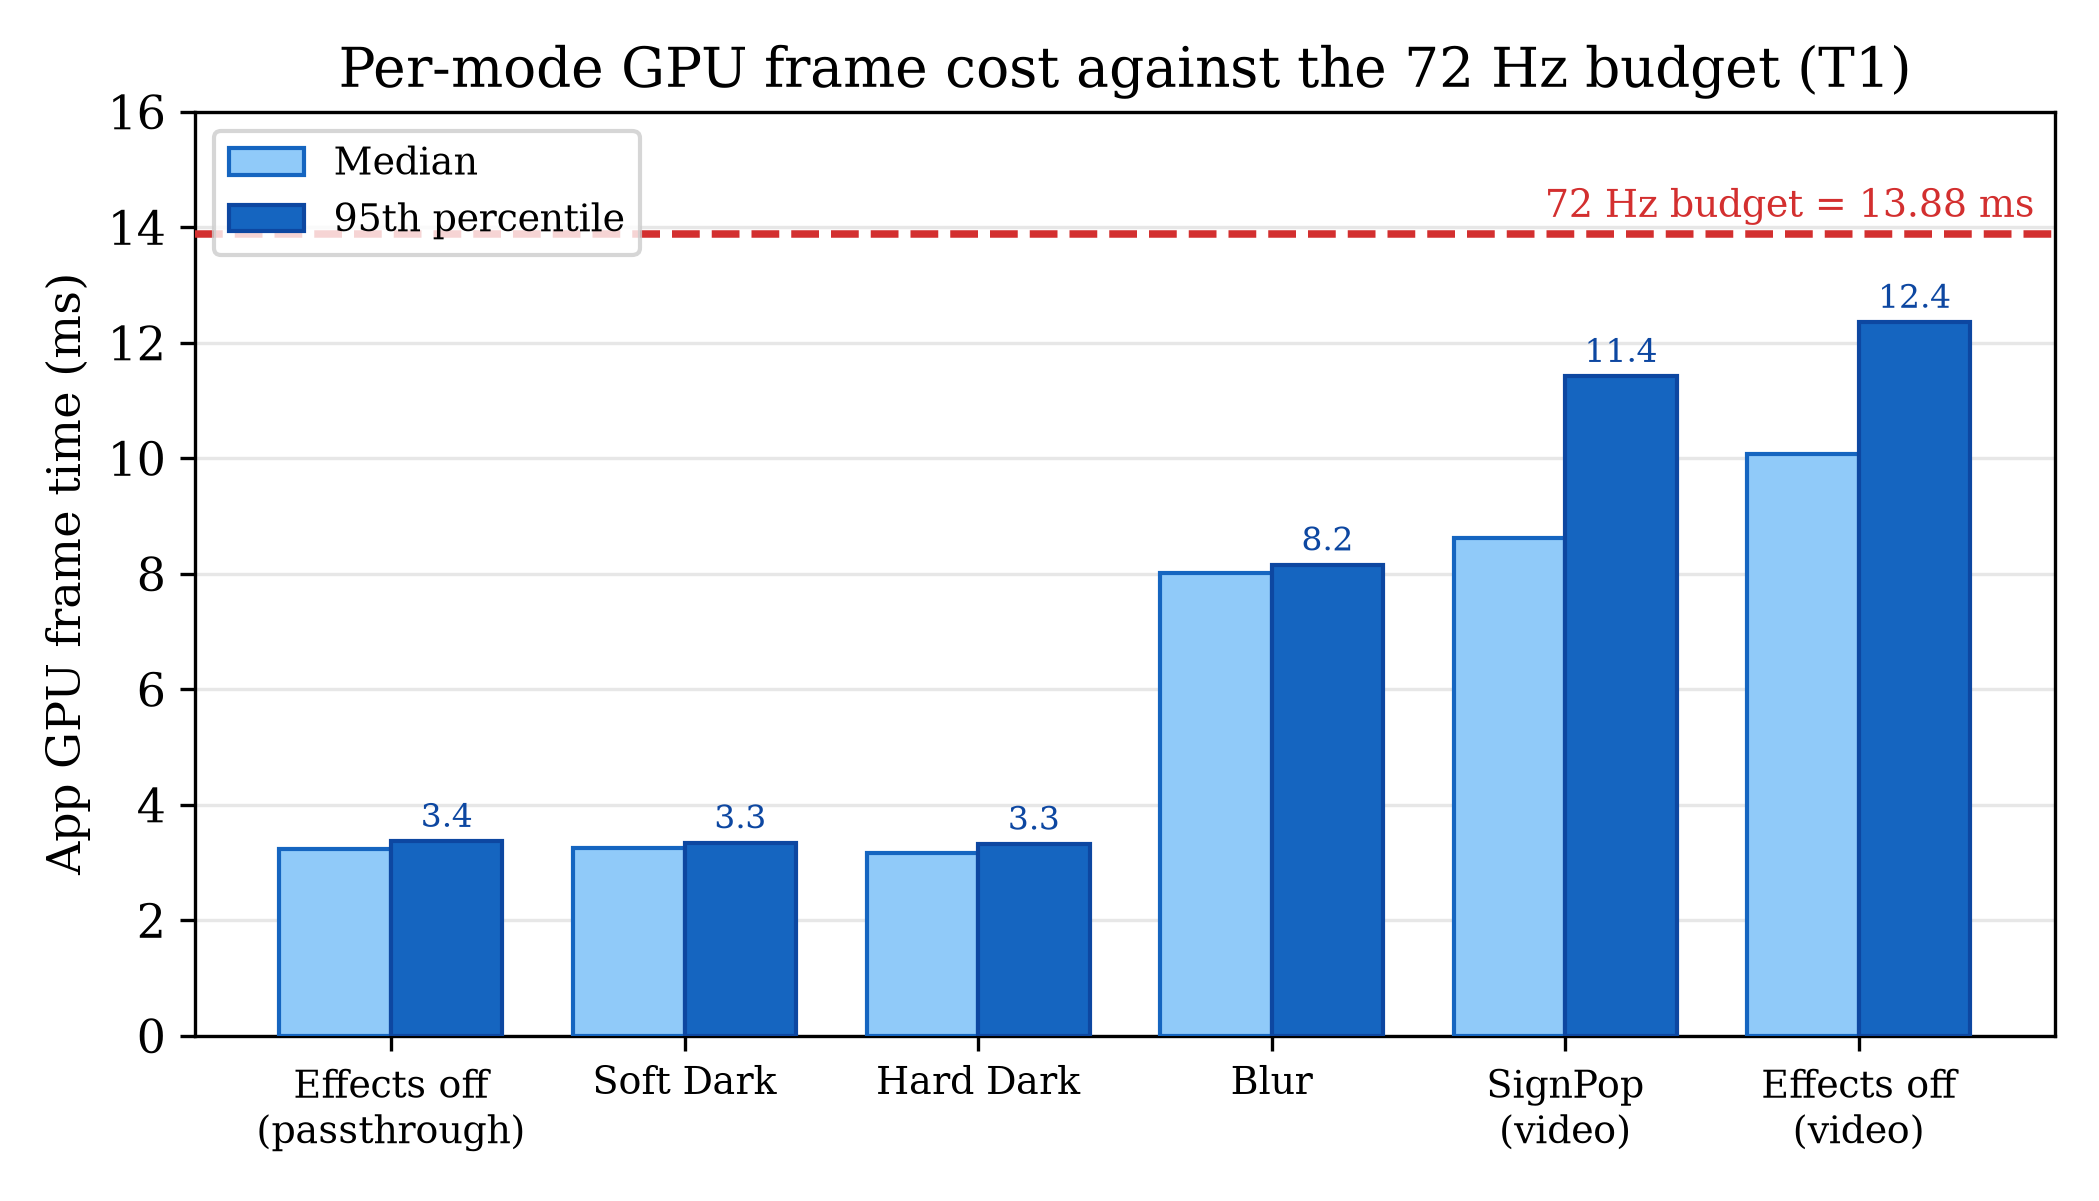
\includegraphics[width=\linewidth]{content/figures/fig_t1_framecost.png}
\caption{Per-mode GPU frame time against the 72 Hz budget.}
\label{fig:t1}
\end{figure}

Three findings. First, \textbf{the dark modes cost nothing measurable}: their 95th-percentile frame
times sit within 0.05 ms of the empty passthrough scene, at a quarter of the budget, with stale
rates at or near zero. The deployability argument of Chapter 3 is now empirical rather than
structural. Second, \textbf{Blur is the price of Tier-3 re-rendering made visible}: two and a half
times the dark modes' frame time and nearly double the GPU utilisation, yet still comfortably
inside the budget, so the Tier-3 ceiling on this hardware is thermal and sustained-load, not
per-frame. Third, \textbf{the video scene misses the stale-frame criterion, in both arms equally}:
7.3\% with SignPop on and 7.9\% with it off, against the 1\% threshold, while 95th-percentile GPU
time stays inside the budget. The miss is a property of the shared 4K video-decode path, not of the
treatment, and SignPop's own grading adds no stall on top of it. The paired Block B comparison is
therefore undisturbed, since both conditions ride the same pipeline, but the configuration misses
its pre-stated criterion and is reported as missing it.

\subsection{Legibility across the two rendering paths}

The window-as-absence architecture rests on the claim that native passthrough through the window is
visibly better than the camera re-render that Tier 3 could put in its place. To measure it, a
Landolt~C acuity chart covering logMAR 1.3 to 0.0 in 0.1 steps, sized for a 600 mm viewing
distance, was printed at 100\% scale and fixed at 600 mm from the headset, which rested on a stable
support and did not move. A debug toggle switched the whole view between the two paths: native
passthrough, and the full-field camera re-render with the grading neutralised at runtime, so the
comparison isolates the rendering path rather than any mode's styling. Each segment identifies
itself in the recording through an on-screen debug label. The pre-stated criterion: the
architecture is vindicated if the native path resolves at least one logMAR step finer than the
camera path.

A cast recording is a valid instrument here because both paths share everything downstream of the
compositor, so any resolution difference originates upstream and survives into the capture. The
capture (1280$\times$685 per eye) undersamples both paths, the native path far more severely than
the camera path, and the camera path additionally renders the chart larger in frame because the
physical camera sits closer to it than the eye does. Both effects compress or favour the camera
path's side of the difference, so the measured gap is a lower bound on the true one, which is the
right direction for a one-sided criterion. Figure~\ref{fig:t3} shows the same chart through both
paths, from the same recording, seconds apart.

\begin{figure}[htbp]
\centering
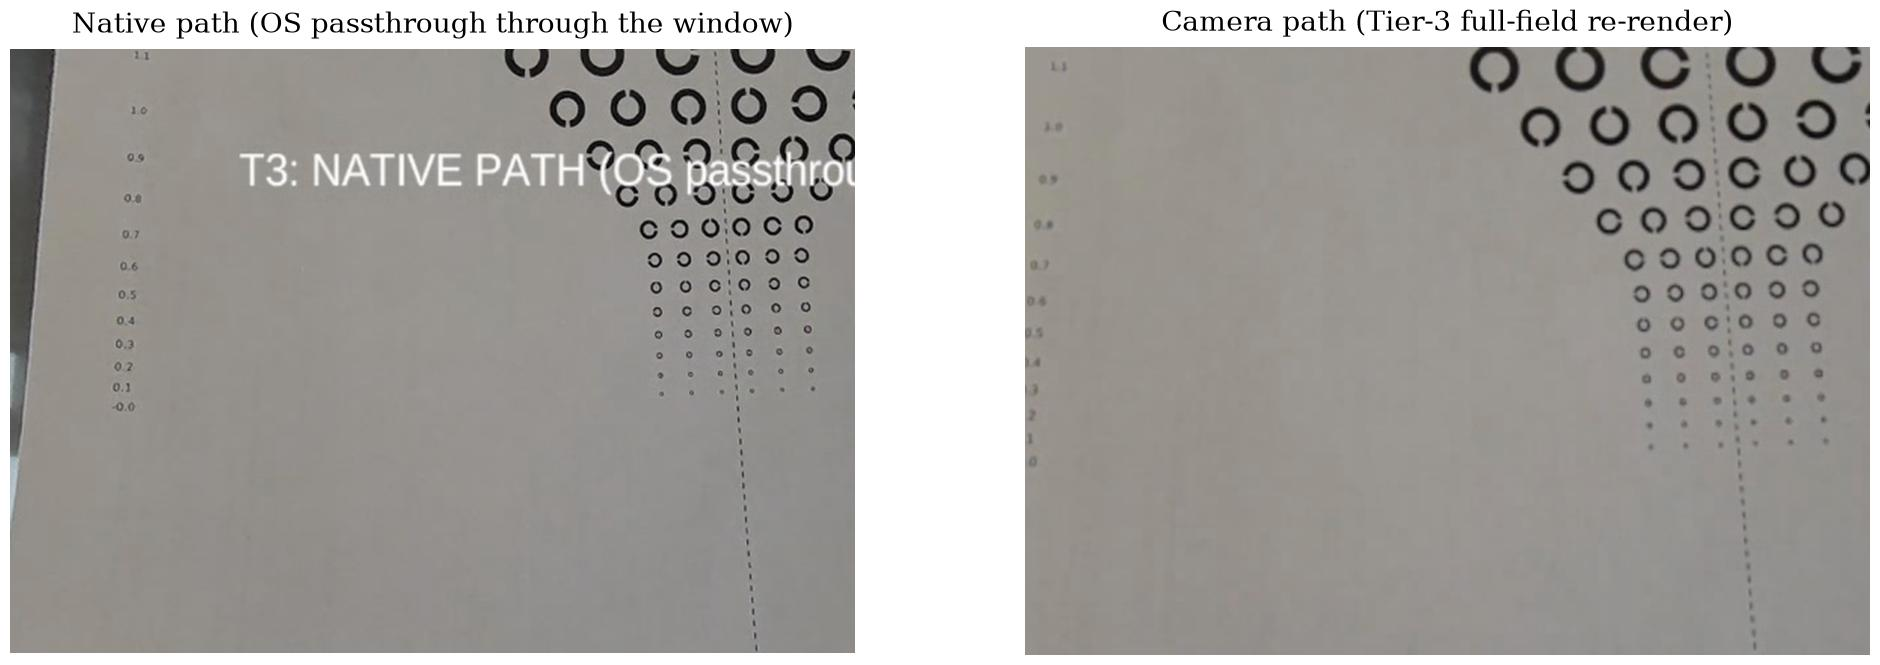
\includegraphics[width=\linewidth]{content/figures/fig_t3_legibility.jpg}
\caption{The Landolt C chart at 600 mm through the two rendering paths, from one continuous cast
recording with the headset stationary. Row labels are logMAR values. The native path holds ring-gap
orientation about two 0.1-logMAR rows further down the chart than the camera path.}
\label{fig:t3}
\end{figure}

\textbf{The criterion is met with margin.} In the capture, the native path holds ring-gap
orientation clearly through the 0.6 row and marginally to 0.5, while the camera path's gaps blur
closed below the 0.8 row. That is a native advantage of at least two 0.1-logMAR steps, roughly a
factor of 1.6 in resolvable detail, despite every capture bias running the other way. The
application's frame-rate overlay held 72 fps in both segments, so neither path bought its
appearance with dropped frames. The limits of the method are stated plainly: one chart, one
distance, one lighting condition, and a legibility read taken from the recording by the author
rather than a psychophysical procedure with naive observers. Within those limits, the measurement
confirms what the architecture bet on, and what \citet{wang2026} measured for passthrough acuity
generally: the place where full pixel control exists is also the place where the image is worst,
and the window spares the focus region exactly that penalty.

\section{Summary}

One sphere, one shader, one manager: the implementation realises Chapter 3's design space with a
per-fragment colour and alpha policy over a world-locked spherical window. Its load-bearing
techniques, the window as absence, the hybrid composite of native passthrough and processed camera
feed, and eye-independent world-direction sampling, are each answers to a specific platform wall, and
its failures are documented with the same care as its successes because both are findings about
building DR on consumer hardware. Its two central trade-offs are measured on device: the dark modes cost
nothing over an empty scene, and the native path the window preserves resolves at least two logMAR
steps finer than the camera copy. Chapter 5 asks whether any of it helps a person.
